\documentclass[12pt]{article}

\usepackage[a4paper, margin=1in]{geometry}
\usepackage{amsmath, amssymb, amsfonts}
\usepackage{graphicx}
\usepackage{booktabs}
\usepackage{hyperref}
\usepackage{natbib}
\usepackage{setspace}

\onehalfspacing

\title{Volatility as an Asset Class: Variance Swaps, VIX Options, and the Volatility Risk Premium}
\author{Group 4}
\date{\today}

\begin{document}

\maketitle

\begin{abstract}
This paper studies volatility as a tradable asset class through variance swaps, VIX options, and the volatility risk premium. The project combines theoretical derivations, Monte Carlo simulation, Fourier/COS pricing, and later empirical validation using market data.
\end{abstract}

\section{Introduction}
\label{sec:introduction}

Volatility plays a central role in modern financial markets. In its most basic interpretation, volatility measures the uncertainty of asset returns. In derivative pricing, however, volatility is more than a statistical input: it becomes a risk factor, a market expectation, and in many cases a directly tradable quantity. Products such as variance swaps, VIX futures, and VIX options allow investors to take positions on future realised or implied volatility without necessarily taking a direct directional position in the underlying equity index.

The development of volatility-linked derivatives has changed the way market participants understand and manage risk. A variance swap, for example, provides exposure to realised variance over a fixed time interval. VIX futures and VIX options provide exposure to market expectations of future volatility. These instruments are widely used for hedging, speculation, relative value trading, and volatility risk premium strategies. Their pricing therefore requires a framework that connects stochastic variance dynamics, risk-neutral valuation, numerical approximation, and empirical validation.

The main objective of this project is to study volatility as an asset class through variance swaps and VIX-linked derivatives. The project develops a quantitative framework that combines theoretical derivations with numerical pricing methods. The theoretical part is based on a Heston-type stochastic volatility model, where the instantaneous variance follows a Cox--Ingersoll--Ross square-root process. This model is useful as a benchmark because it captures mean reversion in variance while preserving a level of analytical tractability.

The project is organised around four completed components. The first component reviews the literature on volatility derivatives, variance risk premia, stochastic volatility models, and recent numerical methods. The second component develops the mathematical framework, including the variance swap strike, the model-implied VIX proxy, and the characteristic function of terminal CIR variance. The third component implements a Monte Carlo engine for Heston simulation, realised variance estimation, variance swap validation, and model-implied VIX call pricing. The fourth component implements a Fourier-cosine pricing engine for VIX derivatives using the characteristic function of terminal variance.

The numerical part of the project is deliberately built around two complementary methods. Monte Carlo simulation is flexible and intuitive. It allows stock and variance paths to be generated directly and can be used for path-dependent quantities such as realised variance. Its main limitation is that it contains sampling error and may require many paths for stable estimates. The Fourier-cosine method, in contrast, is deterministic once the model parameters and truncation interval are fixed. It can be computationally efficient when the characteristic function of the relevant state variable is available. The use of both approaches provides a natural cross-validation framework.

A key modelling distinction in this project is the difference between the official Cboe VIX index and the model-implied VIX proxy used in the numerical implementation. The official VIX is computed from a strip of out-of-the-money SPX option prices according to the Cboe methodology. The proxy used in this project is instead derived from the conditional expectation of future variance under the Heston model. Therefore, the project does not claim to reproduce the exchange methodology exactly. Rather, it studies a Heston-implied VIX-type quantity that is mathematically convenient for pricing and validation.

The research contribution of the current implementation is not a new stochastic volatility model, but a structured numerical framework that connects the theory and implementation of volatility-linked derivatives. The Monte Carlo engine provides a simulation-based estimate of realised variance and VIX option payoffs. The COS engine provides a characteristic-function-based benchmark. The comparison between the two engines helps verify whether the implementation is internally consistent.

The rest of the paper is structured as follows. Section~\ref{sec:literature_review} reviews the relevant literature and recent methodological developments. Section~\ref{sec:theory} presents the mathematical framework. Section~\ref{sec:monte_carlo} develops the Monte Carlo methodology. Section~\ref{sec:cos_pricing} presents the CIR-based COS pricing engine. The later sections discuss numerical validation, code architecture, limitations, and future extensions toward real data calibration and volatility risk premium backtesting.
The Heston model is a central benchmark in stochastic volatility modelling because it introduces a mean-reverting square-root variance process while preserving a degree of analytical tractability. In this framework, the variance process follows a Cox--Ingersoll--Ross type dynamics. This makes it suitable for both Monte Carlo simulation and characteristic-function-based pricing \citep{hirsa2024}.

Recent work also emphasises the importance of numerical accuracy in both simulation-based and transform-based pricing methods. In particular, recent studies on the COS method show that the truncation interval and the number of cosine terms are central numerical choices rather than secondary implementation details \citep{junike2022cos,junike2024cos}.
\section{Mathematical Framework}
\label{sec:theory}

This section presents the mathematical framework used in the project. The objective is to define the stochastic volatility model, derive the variance swap benchmark, construct the model-implied VIX proxy, and introduce the characteristic function of terminal CIR variance. These results provide the theoretical basis for the Monte Carlo engine in Section~\ref{sec:monte_carlo} and the COS pricing engine in Section~\ref{sec:cos_pricing}.

\subsection{Risk-Neutral Pricing Principle}

Derivative prices in this project are computed under the risk-neutral measure \(\mathbb{Q}\). If a derivative pays a terminal payoff \(\Phi\) at maturity \(T\), its time-zero price is given by
\begin{equation}
V_0
=
e^{-rT}
\mathbb{E}^{\mathbb{Q}}
\left[
\Phi
\right],
\end{equation}
where \(r\) is the continuously compounded risk-free rate. This representation is the common foundation for both simulation-based and transform-based pricing. Monte Carlo approximates the expectation by averaging simulated payoffs, while the COS method approximates the same expectation using the characteristic function of the state variable.

In the present setting, the payoff may depend on realised variance, terminal variance, or a model-implied VIX level. The choice of state variable determines which numerical method is more convenient. Path-dependent quantities, such as realised variance, are naturally handled by Monte Carlo simulation. Payoffs depending on terminal variance are suitable for characteristic-function-based methods because terminal CIR variance has a known transform.

\subsection{Heston Stochastic Volatility Model}

The project uses the Heston stochastic volatility model as the baseline framework. Under the risk-neutral measure \(\mathbb{Q}\), the asset price \(S_t\) and instantaneous variance \(v_t\) satisfy
\begin{align}
\frac{dS_t}{S_t}
&=
r\,dt+\sqrt{v_t}\,dW_t^S, \label{eq:heston_stock}\\
dv_t
&=
\kappa(\theta-v_t)\,dt+\sigma_v\sqrt{v_t}\,dW_t^v, \label{eq:heston_variance}\\
d\langle W^S,W^v\rangle_t
&=
\rho\,dt. \label{eq:heston_corr}
\end{align}
Here, \(r\) is the risk-free rate, \(\kappa>0\) is the speed of mean reversion, \(\theta>0\) is the long-run variance level, \(\sigma_v>0\) is the volatility of variance, and \(\rho\in[-1,1]\) is the correlation between the stock and variance shocks.

The variance process in \eqref{eq:heston_variance} is a Cox--Ingersoll--Ross process. Its drift term \(\kappa(\theta-v_t)\) pulls variance toward the long-run level \(\theta\). If \(v_t>\theta\), the drift is negative and variance tends to decrease. If \(v_t<\theta\), the drift is positive and variance tends to increase. This mean-reverting structure is important for the model-implied VIX term structure.

The diffusion term \(\sigma_v\sqrt{v_t}\,dW_t^v\) makes the variance stochastic. The square-root specification ensures that the diffusion coefficient decreases as variance approaches zero. In continuous time, the process is non-negative under standard parameter conditions. In numerical simulation, however, discrete approximations may still produce small negative values, which motivates the use of full-truncation Euler simulation in the Monte Carlo engine.

\subsection{Conditional Mean of the CIR Variance Process}

A central quantity used throughout the project is the conditional expectation of future variance. Taking expectation in the CIR variance equation gives the ordinary differential equation
\begin{equation}
\frac{d}{dt}\mathbb{E}^{\mathbb{Q}}[v_t]
=
\kappa
\left(
\theta-\mathbb{E}^{\mathbb{Q}}[v_t]
\right).
\end{equation}
Solving this equation with initial value \(v_0\) gives
\begin{equation}
\mathbb{E}^{\mathbb{Q}}[v_t]
=
\theta+(v_0-\theta)e^{-\kappa t}.
\label{eq:cir_mean}
\end{equation}
More generally, conditional on information at time \(t\),
\begin{equation}
\mathbb{E}^{\mathbb{Q}}_t[v_{t+u}]
=
\theta+(v_t-\theta)e^{-\kappa u}.
\label{eq:conditional_cir_mean}
\end{equation}

This formula is used twice in the project. First, it gives the analytical variance swap strike. Second, it gives the affine representation of the model-implied VIX proxy.

\subsection{Variance Swap Strike}

A variance swap is a contract whose payoff depends on realised variance over a fixed interval. In continuous time, the idealised floating leg is based on average integrated variance:
\begin{equation}
\frac{1}{T}\int_0^T v_s\,ds.
\end{equation}
The fair variance swap strike is therefore defined as the risk-neutral expectation of this quantity:
\begin{equation}
K_{\mathrm{var}}(0,T)
=
\frac{1}{T}
\mathbb{E}^{\mathbb{Q}}
\left[
\int_0^T v_s\,ds
\right].
\label{eq:kvar_definition}
\end{equation}

Using Fubini's theorem and the conditional mean in \eqref{eq:cir_mean}, we obtain
\begin{align}
K_{\mathrm{var}}(0,T)
&=
\frac{1}{T}
\int_0^T
\mathbb{E}^{\mathbb{Q}}[v_s]\,ds \\
&=
\frac{1}{T}
\int_0^T
\left[
\theta+(v_0-\theta)e^{-\kappa s}
\right]ds.
\end{align}
Evaluating the integral yields
\begin{equation}
\boxed{
K_{\mathrm{var}}(0,T)
=
\theta+
(v_0-\theta)
\frac{1-e^{-\kappa T}}{\kappa T}.
}
\label{eq:kvar_closed_form}
\end{equation}

This expression is important because it provides a closed-form benchmark. In the Monte Carlo part, the simulated realised variance is compared with \eqref{eq:kvar_closed_form}. If the simulation is implemented correctly and the number of paths is sufficiently large, the Monte Carlo mean should be close to the analytical strike.

\subsection{Realised Variance and Its Discrete Approximation}

In the numerical implementation, realised variance is computed from simulated stock prices observed on a finite time grid
\[
0=t_0<t_1<\cdots<t_m=T.
\]
The annualised realised variance estimator is
\begin{equation}
\widehat{\mathrm{RV}}_{0,T}^{(m)}
=
\frac{1}{T}
\sum_{i=1}^{m}
\left(
\log\frac{S_{t_i}}{S_{t_{i-1}}}
\right)^2.
\label{eq:rv_discrete}
\end{equation}
This is the discrete analogue of quadratic variation. Under a continuous diffusion model, as the time mesh becomes finer, the sum of squared log returns approximates the integrated variance:
\begin{equation}
\widehat{\mathrm{RV}}_{0,T}^{(m)}
\rightarrow
\frac{1}{T}
\int_0^T v_s\,ds.
\label{eq:rv_limit}
\end{equation}

This connection justifies comparing simulated realised variance with the analytical variance swap strike. The realised variance estimator is path-based, while \(K_{\mathrm{var}}\) is expectation-based. Therefore, the comparison is performed after averaging realised variance across many Monte Carlo paths.

\subsection{Model-Implied VIX Proxy}

The official VIX index is constructed from SPX option prices, but the project uses a model-implied VIX proxy derived from expected future variance. For a fixed window \(\Delta\), the model-implied VIX at time \(T\) is defined by
\begin{equation}
\widetilde{\mathrm{VIX}}_T^2
=
100^2
\frac{1}{\Delta}
\mathbb{E}^{\mathbb{Q}}_T
\left[
\int_T^{T+\Delta}v_s\,ds
\right].
\label{eq:vix_proxy_definition}
\end{equation}
The factor \(100^2\) converts variance units into VIX index-point units.

Using the conditional mean \eqref{eq:conditional_cir_mean}, we have
\begin{align}
\frac{1}{\Delta}
\mathbb{E}^{\mathbb{Q}}_T
\left[
\int_T^{T+\Delta}v_s\,ds
\right]
&=
\frac{1}{\Delta}
\int_0^\Delta
\mathbb{E}^{\mathbb{Q}}_T[v_{T+u}]\,du \\
&=
\frac{1}{\Delta}
\int_0^\Delta
\left[
\theta+(v_T-\theta)e^{-\kappa u}
\right]du.
\end{align}
Evaluating the integral gives
\begin{equation}
\frac{1}{\Delta}
\mathbb{E}^{\mathbb{Q}}_T
\left[
\int_T^{T+\Delta}v_s\,ds
\right]
=
\theta+(v_T-\theta)
\frac{1-e^{-\kappa\Delta}}{\kappa\Delta}.
\end{equation}
Define
\begin{align}
B_\Delta
&=
\frac{1-e^{-\kappa\Delta}}{\kappa\Delta},
\label{eq:b_delta}\\
A_\Delta
&=
\theta(1-B_\Delta).
\label{eq:a_delta}
\end{align}
Then the model-implied VIX proxy can be written as
\begin{equation}
\boxed{
\widetilde{\mathrm{VIX}}_T
=
100\sqrt{A_\Delta+B_\Delta v_T}.
}
\label{eq:vix_affine}
\end{equation}

The relation in \eqref{eq:vix_affine} is central for both the Monte Carlo and COS pricing engines. In Monte Carlo, terminal variance is simulated path by path and then converted into VIX. In the COS method, the payoff becomes a deterministic function of terminal variance, which allows the terminal CIR characteristic function to be used.

\subsection{Terminal CIR Distribution}

For the COS pricing engine, the relevant state variable is terminal variance \(v_T\). The CIR process has a known terminal distribution:
\begin{equation}
v_T
\sim
c_T\chi_d^2(\lambda_T),
\label{eq:cir_terminal_dist}
\end{equation}
where
\begin{align}
c_T
&=
\frac{\sigma_v^2(1-e^{-\kappa T})}{4\kappa},
\label{eq:c_t}\\
d
&=
\frac{4\kappa\theta}{\sigma_v^2},
\label{eq:d_cir}\\
\lambda_T
&=
\frac{4\kappa e^{-\kappa T}v_0}
{\sigma_v^2(1-e^{-\kappa T})}.
\label{eq:lambda_t}
\end{align}
Here, \(d\) is the degrees-of-freedom parameter and \(\lambda_T\) is the noncentrality parameter.

The characteristic function of \(v_T\) is therefore
\begin{equation}
\boxed{
\varphi_{v_T}(u)
=
(1-2iu c_T)^{-d/2}
\exp\left(
\frac{iu c_T\lambda_T}{1-2iu c_T}
\right).
}
\label{eq:terminal_cir_cf}
\end{equation}
This is different from the transform of integrated variance. The distinction is important because the variance swap depends on \(\int_0^T v_s\,ds\), while the model-implied VIX payoff in this project depends on terminal variance \(v_T\) through \eqref{eq:vix_affine}.

\subsection{Pricing Implications}

The formulas above determine the roles of the two numerical engines. The Monte Carlo engine is used when path simulation is natural, particularly for realised variance. The COS engine is used when the payoff can be written as a function of terminal variance and the characteristic function is available.

For a model-implied VIX call with strike \(K\), the payoff is
\begin{equation}
g_{\mathrm{call}}(v_T)
=
\left(
100\sqrt{A_\Delta+B_\Delta v_T}-K
\right)^+.
\label{eq:vix_call_payoff}
\end{equation}
This payoff can be priced either by Monte Carlo simulation or by the COS method. The agreement between the two pricing approaches provides a consistency check for the implementation.
\section{Monte Carlo Framework}
\label{sec:monte_carlo}

This section describes the Monte Carlo component of the project. The purpose of the W3 implementation is to simulate the Heston stochastic volatility model, estimate realised variance from simulated asset paths, validate the simulation against the analytical Heston variance swap strike, and price a model-implied VIX call option. Monte Carlo simulation is used because it provides a flexible numerical approximation of risk-neutral expectations and can be applied directly to path-dependent quantities such as realised variance \citep{hirsa2024}.

The Monte Carlo engine also serves as an independent benchmark for the Fourier-cosine pricing method developed in Section~\ref{sec:cos_pricing}. While the COS method is deterministic and based on the terminal variance characteristic function, Monte Carlo uses simulated paths and therefore contains sampling and discretisation error. Comparing the two methods under the same parameter set provides a useful internal validation check.

\subsection{Simulation Objective}

The Monte Carlo implementation has three main objectives. First, it generates joint paths of the asset price \(S_t\) and variance \(v_t\) under the risk-neutral Heston dynamics. Second, it computes realised variance from simulated log returns and compares the average realised variance with the analytical variance swap strike. Third, it prices a model-implied VIX call option by transforming terminal variance into a VIX proxy and averaging discounted payoffs.

The simulation is performed under the risk-neutral measure \(\mathbb{Q}\), because derivative prices are represented as discounted risk-neutral expectations. For a terminal payoff \(\Phi\), the general pricing relation is
\begin{equation}
V_0
=
e^{-rT}
\mathbb{E}^{\mathbb{Q}}[\Phi].
\end{equation}
Monte Carlo approximates this expectation by simulating \(N\) independent paths and computing the sample average:
\begin{equation}
V_0^{MC}
=
e^{-rT}
\frac{1}{N}
\sum_{j=1}^{N}
\Phi^{(j)}.
\end{equation}

\subsection{Heston Path Simulation}

The simulated model is the risk-neutral Heston system:
\begin{align}
\frac{dS_t}{S_t}
&=
r\,dt+\sqrt{v_t}\,dW_t^S,\\
dv_t
&=
\kappa(\theta-v_t)\,dt+\sigma_v\sqrt{v_t}\,dW_t^v,\\
d\langle W^S,W^v\rangle_t
&=
\rho\,dt.
\end{align}
The correlation between the Brownian motions is implemented by generating two independent standard normal variables \(Z_v\) and \(Z_\perp\), and then defining
\begin{equation}
Z_S
=
\rho Z_v+\sqrt{1-\rho^2}\,Z_\perp.
\end{equation}
This construction ensures that
\begin{equation}
\operatorname{Corr}(Z_S,Z_v)=\rho.
\end{equation}

The time interval \([0,T]\) is divided into \(m\) equal steps of length
\begin{equation}
\Delta t=\frac{T}{m}.
\end{equation}
The simulation stores both the stock paths and the variance paths. The stock paths are used to compute realised variance, while the terminal variance values are used for model-implied VIX pricing.

\subsection{Full-Truncation Euler Scheme}

The variance process contains the square-root term \(\sqrt{v_t}\). In continuous time, the CIR process is non-negative under standard conditions. However, in discrete-time numerical simulation, a simple Euler update may produce negative variance values. Since \(\sqrt{v_t}\) is not defined for negative \(v_t\), a stability correction is required.

The implementation uses a full-truncation Euler scheme. Define
\begin{equation}
v_t^+
=
\max(v_t,0).
\end{equation}
The variance update is
\begin{equation}
v_{t+\Delta t}
=
v_t
+
\kappa(\theta-v_t^+)\Delta t
+
\sigma_v\sqrt{v_t^+}\sqrt{\Delta t}\,Z_v.
\label{eq:mc_variance_update}
\end{equation}
After the update, the next variance value is floored at zero:
\begin{equation}
v_{t+\Delta t}
\leftarrow
\max(v_{t+\Delta t},0).
\end{equation}

The stock price is simulated in logarithmic form:
\begin{equation}
\log S_{t+\Delta t}
=
\log S_t
+
\left(r-\frac{1}{2}v_t^+\right)\Delta t
+
\sqrt{v_t^+}\sqrt{\Delta t}\,Z_S.
\label{eq:mc_stock_update}
\end{equation}
The log update preserves positivity of the simulated stock price and is consistent with the diffusion form of the asset dynamics.

The simulation of square-root processes requires careful treatment near the zero boundary. Recent work on Heston and related square-root processes emphasises that discretisation choices can materially affect pricing accuracy, especially for variance-sensitive products \citep{choikwok2024heston,abijaber2024squareroot}. The full-truncation scheme is therefore used as a practical balance between numerical stability and implementation simplicity.

\subsection{Realised Variance Estimation}

After simulating stock paths, realised variance is computed from discrete log returns. For a path observed at time points
\[
0=t_0<t_1<\cdots<t_m=T,
\]
the realised variance estimator is
\begin{equation}
\widehat{\mathrm{RV}}_{0,T}^{(j)}
=
\frac{1}{T}
\sum_{i=1}^{m}
\left(
\log\frac{S_{t_i}^{(j)}}{S_{t_{i-1}}^{(j)}}
\right)^2,
\label{eq:mc_realised_variance}
\end{equation}
where \(j\) indexes the simulated path.

The Monte Carlo estimate of expected realised variance is the sample mean:
\begin{equation}
\overline{\mathrm{RV}}_{0,T}^{MC}
=
\frac{1}{N}
\sum_{j=1}^{N}
\widehat{\mathrm{RV}}_{0,T}^{(j)}.
\end{equation}
As the time discretisation becomes finer, realised variance approximates average integrated variance:
\begin{equation}
\widehat{\mathrm{RV}}_{0,T}^{(j)}
\approx
\frac{1}{T}
\int_0^T v_s^{(j)}\,ds.
\end{equation}
Therefore, the Monte Carlo mean should approximate the analytical variance swap strike:
\begin{equation}
\overline{\mathrm{RV}}_{0,T}^{MC}
\approx
K_{\mathrm{var}}(0,T).
\end{equation}

This comparison is the first validation test for the simulation engine. If the Monte Carlo mean realised variance is close to the analytical strike, the simulated variance dynamics are consistent with the theoretical expectation of integrated variance.

\subsection{Variance Swap Benchmark}

The analytical Heston variance swap strike is
\begin{equation}
K_{\mathrm{var}}(0,T)
=
\theta+
(v_0-\theta)
\frac{1-e^{-\kappa T}}{\kappa T}.
\end{equation}
The Monte Carlo engine compares this value with the mean realised variance. The error can be reported as an absolute error,
\begin{equation}
\mathrm{AbsError}_{RV}
=
\left|
\overline{\mathrm{RV}}_{0,T}^{MC}
-
K_{\mathrm{var}}(0,T)
\right|,
\end{equation}
or as a relative error,
\begin{equation}
\mathrm{RelError}_{RV}
=
\frac{
\left|
\overline{\mathrm{RV}}_{0,T}^{MC}
-
K_{\mathrm{var}}(0,T)
\right|
}{
K_{\mathrm{var}}(0,T)
}.
\end{equation}

This benchmark is useful because it checks the numerical implementation against a closed-form theoretical quantity. It does not require market data and can therefore be performed before calibration.

\subsection{Model-Implied VIX Call Pricing}

The second pricing task in the Monte Carlo engine is a model-implied VIX call. The project uses the Heston-implied VIX proxy
\begin{equation}
\widetilde{\mathrm{VIX}}_T
=
100\sqrt{A_\Delta+B_\Delta v_T}.
\end{equation}
For each simulated path \(j\), terminal variance \(v_T^{(j)}\) is transformed into terminal model-implied VIX:
\begin{equation}
\widetilde{\mathrm{VIX}}_T^{(j)}
=
100\sqrt{A_\Delta+B_\Delta v_T^{(j)}}.
\end{equation}
The call payoff is
\begin{equation}
\Phi^{(j)}
=
\left(
\widetilde{\mathrm{VIX}}_T^{(j)}
-
K
\right)^+.
\end{equation}
The Monte Carlo call price is then
\begin{equation}
C_0^{MC}(K,T)
=
e^{-rT}
\frac{1}{N}
\sum_{j=1}^{N}
\left(
100\sqrt{A_\Delta+B_\Delta v_T^{(j)}}
-
K
\right)^+.
\label{eq:mc_vix_call}
\end{equation}

This pricing method is straightforward because it only requires terminal variance values. However, since the terminal variance values come from discretised Heston paths, the result may contain both sampling error and time-discretisation bias.

\subsection{Monte Carlo Confidence Interval}

The uncertainty of the Monte Carlo estimate is measured by the standard error. Let
\[
Y_j
=
e^{-rT}
\left(
100\sqrt{A_\Delta+B_\Delta v_T^{(j)}}
-
K
\right)^+
\]
be the discounted payoff on path \(j\). The Monte Carlo price is
\begin{equation}
C_0^{MC}
=
\frac{1}{N}
\sum_{j=1}^{N}Y_j.
\end{equation}
The sample standard deviation is
\begin{equation}
s_Y
=
\sqrt{
\frac{1}{N-1}
\sum_{j=1}^{N}
\left(
Y_j-C_0^{MC}
\right)^2
}.
\end{equation}
The standard error is
\begin{equation}
SE(C_0^{MC})
=
\frac{s_Y}{\sqrt{N}}.
\end{equation}
An approximate \(95\%\) confidence interval is
\begin{equation}
C_0^{MC}
\pm
1.96\,SE(C_0^{MC}).
\end{equation}

This interval helps interpret the difference between Monte Carlo and COS prices. A small difference between the two methods is meaningful only when the Monte Carlo uncertainty is sufficiently controlled.

\subsection{Convergence Behaviour}

Monte Carlo convergence is governed by the central limit theorem. The sampling error decreases at the rate
\begin{equation}
O(N^{-1/2}),
\end{equation}
where \(N\) is the number of simulated paths. This rate is independent of the dimension of the simulated process, which is one reason Monte Carlo is widely used in finance. However, the convergence is relatively slow: reducing the standard error by a factor of two requires approximately four times as many paths.

The implementation therefore studies price stability across different path counts. In addition to increasing \(N\), time-discretisation error can be reduced by increasing the number of time steps \(m\). In practice, both sources of error must be considered. A large number of paths does not eliminate bias caused by a coarse time grid.

\subsection{Interpretation of W3 Results}

The W3 component provides a flexible simulation-based pricing framework. Its first validation step is the comparison between simulated realised variance and the analytical variance swap strike. Its second output is a Monte Carlo price for a model-implied VIX call. These two tasks show that the engine can be used both for path-based quantities and terminal-payoff derivatives.

The Monte Carlo engine is not intended to be the fastest pricing method in the project. Instead, its role is to provide a transparent and flexible benchmark. It is especially useful because the simulated paths can later be reused for additional tasks such as scenario analysis, preliminary variance-risk comparisons, and empirical extensions once market data are added.

\subsection{Limitations of the Monte Carlo Engine}

The current Monte Carlo implementation has several limitations. First, it uses an Euler-type discretisation rather than exact simulation of the CIR process. This is practical and stable, but it may introduce discretisation bias. Second, the current implementation uses synthetic parameters rather than calibrated market parameters. Third, the VIX quantity priced in the simulation is a Heston-implied proxy rather than the official Cboe VIX index.

These limitations do not invalidate the W3 implementation. Rather, they define the scope of the current stage. The goal of W3 is to build and validate a simulation engine under controlled model assumptions. Future stages can extend this engine by adding market calibration, exact CIR sampling, variance risk premium backtesting, and real-data validation.
\section{CIR-Based COS Pricing Framework}
\label{sec:cos_pricing}

This section presents the Fourier-cosine pricing component of the project. The purpose of the W4 implementation is to provide a deterministic semi-analytical pricing engine for model-implied VIX derivatives. Unlike Monte Carlo simulation, which estimates expectations through random sampling, the COS method approximates the pricing integral using the characteristic function of the relevant state variable. In this project, the state variable is the terminal CIR variance \(v_T\).

Fourier-based pricing methods are useful when the characteristic function is available even if the transition density is not directly used in closed form \citep{hirsa2024}. The COS method is particularly attractive because it approximates the density and expected payoff through a finite cosine expansion. Recent work on the COS method emphasises that both the truncation interval and the number of cosine terms are central numerical choices for pricing accuracy \citep{junike2022cos,junike2024cos}.

\subsection{Purpose of the COS Engine}

The COS engine has three main purposes in the project. First, it provides a pricing method for VIX call and put options under the model-implied VIX proxy. Second, it gives a deterministic benchmark for the Monte Carlo VIX call price from Section~\ref{sec:monte_carlo}. Third, it supports additional validation through density recovery and convergence checks.

The method is well suited to the present setting because the terminal variance \(v_T\) has a known characteristic function under the CIR process. Since the model-implied VIX is written as
\begin{equation}
\widetilde{\mathrm{VIX}}_T
=
100\sqrt{A_\Delta+B_\Delta v_T},
\end{equation}
a VIX derivative payoff can be treated as a deterministic function of terminal variance. This allows pricing to be formulated as an expectation over \(v_T\).

\subsection{Terminal CIR Characteristic Function}

The variance process in the Heston model follows the CIR dynamics
\begin{equation}
dv_t
=
\kappa(\theta-v_t)dt+\sigma_v\sqrt{v_t}\,dW_t^v.
\end{equation}
For maturity \(T\), the terminal variance has the scaled non-central chi-square representation
\begin{equation}
v_T
\sim
c_T\chi_d^2(\lambda_T),
\end{equation}
where
\begin{align}
c_T
&=
\frac{\sigma_v^2(1-e^{-\kappa T})}{4\kappa},\\
d
&=
\frac{4\kappa\theta}{\sigma_v^2},\\
\lambda_T
&=
\frac{4\kappa e^{-\kappa T}v_0}
{\sigma_v^2(1-e^{-\kappa T})}.
\end{align}
The corresponding characteristic function is
\begin{equation}
\boxed{
\varphi_{v_T}(u)
=
(1-2iu c_T)^{-d/2}
\exp\left(
\frac{iu c_T\lambda_T}{1-2iu c_T}
\right).
}
\label{eq:cos_terminal_cf}
\end{equation}

This is the characteristic function used in the COS pricing engine. It is important to distinguish this terminal variance characteristic function from the transform of integrated variance. Variance swaps depend on the integrated variance \(\int_0^T v_s\,ds\), whereas the VIX option payoff in this implementation depends on terminal variance through the model-implied VIX proxy.

\subsection{COS Representation of the Density}

Let \(X\) be a random variable with density \(f_X(x)\) and characteristic function \(\varphi_X(u)\). The COS method approximates the density on a finite interval \([a,b]\) by a Fourier-cosine expansion:
\begin{equation}
f_X(x)
\approx
\sideset{}{'}\sum_{k=0}^{N-1}
A_k
\cos\left(
\frac{k\pi(x-a)}{b-a}
\right),
\label{eq:cos_density_general}
\end{equation}
where the prime indicates that the first term is multiplied by one half. The coefficients are obtained from the characteristic function:
\begin{equation}
A_k
=
\frac{2}{b-a}
\operatorname{Re}
\left[
\varphi_X\left(\frac{k\pi}{b-a}\right)
e^{-ik\pi a/(b-a)}
\right].
\label{eq:cos_density_coefficients}
\end{equation}

In this project, \(X=v_T\), so \(\varphi_X=\varphi_{v_T}\). The approximation in \eqref{eq:cos_density_general} is therefore applied to the terminal CIR variance density. This density recovery is not only useful for interpretation, but also serves as a numerical check that the characteristic function and truncation interval are implemented consistently.

\subsection{COS Pricing Formula}

For a derivative payoff \(g(X)\), the time-zero price under the risk-neutral measure is
\begin{equation}
V_0
=
e^{-rT}
\mathbb{E}^{\mathbb{Q}}[g(X)].
\end{equation}
Using the COS density approximation, this expectation can be approximated as
\begin{equation}
V_0
\approx
e^{-rT}
\sideset{}{'}\sum_{k=0}^{N-1}
\operatorname{Re}
\left[
\varphi_X\left(\frac{k\pi}{b-a}\right)
e^{-ik\pi a/(b-a)}
\right]
G_k,
\label{eq:cos_price_general}
\end{equation}
where
\begin{equation}
G_k
=
\frac{2}{b-a}
\int_a^b
g(x)
\cos\left(
\frac{k\pi(x-a)}{b-a}
\right)
dx
\label{eq:cos_payoff_coefficient}
\end{equation}
is the payoff cosine coefficient.

The expression in \eqref{eq:cos_price_general} is the main pricing formula used by the COS engine. It separates the distributional part, represented by the characteristic function, from the payoff part, represented by \(G_k\). This separation is one of the reasons Fourier-based methods are efficient for repeated pricing across different strikes.

\subsection{VIX Call and Put Payoffs}

In the current implementation, the model-implied VIX proxy is
\begin{equation}
\widetilde{\mathrm{VIX}}_T
=
100\sqrt{A_\Delta+B_\Delta v_T}.
\end{equation}
Therefore, the payoff of a VIX call with strike \(K\) can be written as a function of terminal variance:
\begin{equation}
g_{\mathrm{call}}(v)
=
\left(
100\sqrt{A_\Delta+B_\Delta v}-K
\right)^+.
\label{eq:cos_call_payoff}
\end{equation}
Similarly, the payoff of a VIX put is
\begin{equation}
g_{\mathrm{put}}(v)
=
\left(
K-100\sqrt{A_\Delta+B_\Delta v}
\right)^+.
\label{eq:cos_put_payoff}
\end{equation}

The call and put prices are then computed by substituting these payoff functions into the COS pricing formula. For the call,
\begin{equation}
C_0^{COS}(K,T)
\approx
e^{-rT}
\sideset{}{'}\sum_{k=0}^{N-1}
\operatorname{Re}
\left[
\varphi_{v_T}\left(\frac{k\pi}{b-a}\right)
e^{-ik\pi a/(b-a)}
\right]
G_k^{\mathrm{call}},
\label{eq:cos_call_price}
\end{equation}
where
\begin{equation}
G_k^{\mathrm{call}}
=
\frac{2}{b-a}
\int_a^b
\left(
100\sqrt{A_\Delta+B_\Delta v}-K
\right)^+
\cos\left(
\frac{k\pi(v-a)}{b-a}
\right)
dv.
\end{equation}
The put price is computed analogously:
\begin{equation}
P_0^{COS}(K,T)
\approx
e^{-rT}
\sideset{}{'}\sum_{k=0}^{N-1}
\operatorname{Re}
\left[
\varphi_{v_T}\left(\frac{k\pi}{b-a}\right)
e^{-ik\pi a/(b-a)}
\right]
G_k^{\mathrm{put}}.
\label{eq:cos_put_price}
\end{equation}

In the current implementation, the payoff coefficients are computed numerically. This is practical because the VIX payoff contains a square-root transformation of terminal variance. Closed-form payoff coefficients may be considered in future work to improve computational efficiency.

\subsection{Truncation Interval}

A central practical issue in the COS method is the selection of the truncation interval \([a,b]\). Since CIR variance is non-negative, the lower bound is chosen as
\begin{equation}
a=0.
\end{equation}
The upper bound is selected using the mean and standard deviation of terminal variance:
\begin{equation}
b
=
\mathbb{E}^{\mathbb{Q}}[v_T]
+
L\sqrt{\operatorname{Var}^{\mathbb{Q}}(v_T)}.
\label{eq:cos_truncation}
\end{equation}
Here, \(L>0\) controls the width of the interval. In the implementation, \(L=8\) is used as a practical benchmark setting.

The truncation interval is a critical input in the COS method. If the interval is too narrow, relevant probability mass may be excluded. If the interval is too wide, the approximation may become less efficient because the cosine expansion must represent the function over a larger range. For this reason, recent COS-method literature treats interval selection and the number of expansion terms as key accuracy controls \citep{junike2022cos,junike2024cos}.

\subsection{Density Recovery Check}

The COS engine also includes a density recovery check. Using the coefficients in \eqref{eq:cos_density_coefficients}, the recovered terminal variance density is
\begin{equation}
\widehat{f}_{v_T}(v)
=
\sideset{}{'}\sum_{k=0}^{N-1}
A_k
\cos\left(
\frac{k\pi(v-a)}{b-a}
\right).
\label{eq:cos_recovered_density}
\end{equation}
A basic consistency check is that the recovered density integrates approximately to one:
\begin{equation}
\int_a^b
\widehat{f}_{v_T}(v)\,dv
\approx
1.
\end{equation}
The first moment can also be compared with the analytical CIR mean:
\begin{equation}
\mathbb{E}^{\mathbb{Q}}[v_T]
=
\theta+(v_0-\theta)e^{-\kappa T}.
\end{equation}

These checks are important because the COS method relies on both the characteristic function and the truncation interval. A pricing result may appear numerically reasonable even if the recovered density is poorly normalised. Density recovery provides an additional diagnostic tool before interpreting option prices.

\subsection{VIX Futures Term Structure}

The COS framework can also be used to compute a model-implied VIX futures level. Since a futures level is an expected future index level under the risk-neutral measure, the model-implied VIX futures value is
\begin{equation}
F(0,T)
=
\mathbb{E}^{\mathbb{Q}}
\left[
100\sqrt{A_\Delta+B_\Delta v_T}
\right].
\label{eq:vix_futures}
\end{equation}
There is no discount factor in this expression because a futures price is quoted as a forward level rather than as a discounted payoff.

The VIX term structure reflects mean reversion in the CIR variance process. If \(v_0>\theta\), variance is expected to decline toward its long-run level, producing a downward-sloping curve. This corresponds to backwardation. If \(v_0<\theta\), variance is expected to rise toward its long-run level, producing an upward-sloping curve. This corresponds to contango.

\subsection{Convergence with Respect to COS Terms}

The number of COS terms \(N\) controls the resolution of the cosine expansion. A small value of \(N\) may produce a poor approximation, while a very large value increases computation without necessarily improving the result if truncation error dominates. Therefore, the implementation studies convergence by computing prices for increasing values of \(N\).

The expected behaviour is that prices stabilise as \(N\) increases. In practice, this stabilisation must be assessed together with the truncation interval. Increasing \(N\) cannot correct an interval that excludes relevant probability mass. For this reason, the convergence study considers both \(N\) and the truncation-width parameter \(L\).

\subsection{Comparison with Monte Carlo}

The COS price is compared with the Monte Carlo price from Section~\ref{sec:monte_carlo}. The absolute difference is
\begin{equation}
\mathrm{AbsError}
=
\left|
C_0^{COS}
-
C_0^{MC}
\right|,
\end{equation}
and the relative difference is
\begin{equation}
\mathrm{RelError}
=
\frac{
\left|
C_0^{COS}
-
C_0^{MC}
\right|
}{
C_0^{MC}
}.
\end{equation}

This comparison is useful because the two methods have different sources of numerical error. Monte Carlo contains sampling and time-discretisation error. COS contains truncation error and series approximation error. If both methods produce close prices under the same parameter set, the result supports the internal consistency of the numerical implementation.

\subsection{Interpretation of W4 Implementation}

The W4 implementation extends the project from simulation-based pricing to characteristic-function-based pricing. This is an important methodological step because it introduces a deterministic benchmark that can be used for repeated pricing and validation. The COS engine also makes it possible to recover the terminal variance density and to study the model-implied VIX term structure.

The main practical advantage of the COS method is speed once the characteristic function is available. The main practical challenge is numerical accuracy, especially the selection of the truncation interval and the number of expansion terms. The implementation addresses this by including convergence checks and density recovery diagnostics.

\subsection{Limitations of the COS Engine}

The current COS engine has several limitations. First, the payoff coefficients are computed numerically rather than in closed form. This is acceptable for the current implementation but may be less efficient for large-scale surface construction. Second, the method prices derivatives on a Heston-implied VIX proxy, not on the official Cboe VIX index. Third, the one-factor CIR variance process may not be flexible enough to reproduce real VIX futures and options data after calibration.

These limitations define the natural direction for future work. Possible extensions include closed-form or more efficient payoff coefficient computation, adaptive truncation rules, exact CIR sampling for validation, and multi-factor or rough-volatility specifications for better market fit.
\section{Data Collection and Calibration}
\label{sec:data_calibration}

This section extends the project from the theoretical and numerical W3--W4 framework to the empirical components implemented in W5 and W6. The purpose of W5 is to collect and process market data for volatility analysis, while the purpose of W6 is to calibrate the Heston model to SPX implied-volatility information and the VIX futures term structure.

The earlier sections established the model, the Monte Carlo engine, and the CIR-based COS engine. The data and calibration stages connect these tools to market-facing tasks. In particular, W5 introduces realised and implied variance data, while W6 tests whether a one-factor Heston model can fit both SPX and VIX-related instruments simultaneously.

\subsection{W5 Data Collection and Exploratory Analysis}

The W5 component implements the empirical data pipeline used for volatility risk premium analysis and exploratory volatility-market diagnostics. The workflow includes downloading VIX daily index data, downloading SPX market data, obtaining VIX futures settlement data, computing realised variance from SPX returns, computing ex-post volatility risk premium, estimating ex-ante VRP using GARCH(1,1) forecasts, identifying crisis periods, and generating exploratory plots.

The main data inputs are:
\begin{itemize}
    \item VIX index levels;
    \item SPX index prices;
    \item VIX futures settlement data;
    \item a risk-free rate proxy.
\end{itemize}

The W5 pipeline covers the 2019--2024 period. This sample is useful because it contains both relatively calm volatility regimes and major stress episodes, including the 2020 COVID shock and the 2022 inflation shock. As a result, the dataset can be used not only for average behaviour, but also for crisis-regime interpretation.

\subsection{Realised Variance Estimation}

Realised variance is computed from SPX log returns. If \(S_i\) denotes the SPX level at observation time \(i\), the log return is
\begin{equation}
r_i
=
\log\left(
\frac{S_i}{S_{i-1}}
\right).
\end{equation}
The realised variance over a given period is computed as
\begin{equation}
RV_t
=
\sum_i r_i^2.
\end{equation}
Monthly realised variance is annualised where appropriate.

This realised-variance estimate is important because it provides the empirical counterpart to the theoretical integrated variance discussed in earlier sections. In the Monte Carlo part, realised variance was computed from simulated paths. In W5, the same concept is applied to market data using SPX returns.

\subsection{Implied Variance and Volatility Risk Premium}

The project approximates one-month implied variance from the VIX index:
\begin{equation}
IV_t
=
\frac{1}{12}
\left(
\frac{VIX_t}{100}
\right)^2.
\end{equation}
The one-month ex-post volatility risk premium is then computed as
\begin{equation}
VRP_t
=
IV_t
-
RV_{t,t+1M}.
\end{equation}
Equivalently,
\begin{equation}
VRP_t
=
\frac{1}{12}
\left(
\frac{VIX_t}{100}
\right)^2
-
RV_{t,t+1M}.
\end{equation}

A positive volatility risk premium means that implied variance is higher than subsequently realised variance. Economically, this is interpreted as compensation paid by investors who demand protection against future volatility. Sellers of volatility may earn this premium in normal periods, but they are exposed to large losses during market stress.

\subsection{W5 Empirical Findings}

The W5 exploratory analysis confirms several common stylised facts in volatility markets. First, the VIX index rises sharply during market stress. Second, implied variance is usually higher than future realised variance in calm market conditions. Third, the volatility risk premium is generally positive in normal regimes. Fourth, crisis periods can compress or reverse the premium. Finally, VIX and SPX returns are negatively related, especially during stress periods.

These findings are consistent with the interpretation of volatility as an insurance-like asset class. Market participants often pay a premium to protect against volatility spikes and equity drawdowns. This premium can be harvested in calm periods, but it carries crisis risk when realised variance rises sharply.

\subsection{W6 Joint SPX--VIX Calibration}

The W6 component implements a calibration framework for the Heston model. The goal is to test whether one set of Heston parameters can fit both the SPX implied-volatility surface and the VIX futures term structure.

The W6 workflow includes:
\begin{itemize}
    \item the Heston characteristic function for the log-stock process under the risk-neutral measure;
    \item a COS pricer for European SPX calls and puts;
    \item Black--Scholes implied-volatility inversion using Brent's method;
    \item SPX option-chain loading with CSV cache and synthetic SVI fallback;
    \item SPX calibration loss in vega-scaled price units;
    \item VIX futures calibration loss using the W4 COS engine;
    \item a joint SPX/VIX objective with a tunable mixing weight;
    \item a soft Feller-condition penalty;
    \item a two-stage optimiser combining differential evolution and L-BFGS-B.
\end{itemize}

The calibrated Heston parameter vector is
\begin{equation}
\Theta
=
(\kappa,\theta,\sigma_v,\rho,v_0).
\end{equation}
Here, \(\kappa\) controls mean-reversion speed, \(\theta\) is the long-run variance, \(\sigma_v\) is volatility of variance, \(\rho\) is stock-variance correlation, and \(v_0\) is initial variance.

\subsection{Calibration Objective}

Calibration means choosing model parameters so that model prices are close to market observations. A generic least-squares objective can be written as
\begin{equation}
\min_{\Theta}
\sum_{i=1}^{n}
w_i
\left(
P_i^{model}(\Theta)
-
P_i^{market}
\right)^2,
\end{equation}
where \(P_i^{market}\) is the observed market price or implied volatility, \(P_i^{model}(\Theta)\) is the corresponding model output, and \(w_i\) is a weight.

For SPX options, the model is evaluated through a Heston/COS option pricer and compared to the market implied-volatility surface. For VIX futures, the model-implied futures level is computed using the W4 VIX futures engine and compared to the observed futures curve.

The joint calibration objective combines SPX and VIX components:
\begin{equation}
\mathcal{L}_{joint}(\Theta)
=
\alpha \mathcal{L}_{SPX}(\Theta)
+
(1-\alpha)\mathcal{L}_{VIX}(\Theta)
+
\mathcal{P}_{Feller}(\Theta),
\end{equation}
where \(\alpha\in[0,1]\) controls the relative weight of the SPX and VIX markets, and \(\mathcal{P}_{Feller}\) is a soft penalty for violations of the Feller condition.

\subsection{Calibration Setup}

The calibration uses SPX option-chain information, VIX futures, and a flat risk-free rate proxy. The SPX maturity window is restricted to expirations between 14 and 365 days, and the moneyness range is restricted to log-moneyness within approximately \(\pm 0.4\). Only out-of-the-money calls and puts are used.

The Heston parameter bounds are:
\begin{center}
\begin{tabular}{lcc}
\toprule
Parameter & Lower bound & Upper bound \\
\midrule
\(\kappa\) & 0.10 & 15.00 \\
\(\theta\) & 0.005 & 0.250 \\
\(\sigma_v\) & 0.05 & 2.50 \\
\(\rho\) & -0.99 & 0.00 \\
\(v_0\) & 0.005 & 0.500 \\
\bottomrule
\end{tabular}
\end{center}

A soft quadratic penalty is applied when the Feller condition
\begin{equation}
2\kappa\theta \geq \sigma_v^2
\end{equation}
is violated. This does not strictly force the optimiser to remain inside the Feller region, but discourages parameter combinations that strongly violate the non-attainment condition for the zero boundary.

\subsection{Three Calibration Experiments}

W6 compares three calibration settings:
\begin{enumerate}
    \item SPX-only calibration;
    \item VIX-only calibration;
    \item joint SPX--VIX calibration.
\end{enumerate}

The calibrated parameter values are summarised in Table~\ref{tab:w6_calibrated_parameters}.

\begin{table}[htbp]
\centering
\begin{tabular}{lccccc}
\toprule
Calibration & \(\kappa\) & \(\theta\) & \(\sigma_v\) & \(\rho\) & \(v_0\) \\
\midrule
SPX-only & 0.966 & 0.064 & 0.352 & -0.937 & 0.033 \\
VIX-only & 0.209 & 0.250 & 0.050 & -0.700 & 0.005 \\
Joint \((\alpha=0.50)\) & 0.220 & 0.240 & 0.050 & -0.566 & 0.005 \\
\bottomrule
\end{tabular}
\caption{Calibrated Heston parameters under SPX-only, VIX-only, and joint calibration.}
\label{tab:w6_calibrated_parameters}
\end{table}

The calibration error comparison is shown in Table~\ref{tab:w6_calibration_errors}.

\begin{table}[htbp]
\centering
\begin{tabular}{lcc}
\toprule
Calibration & SPX IV RMSE & VIX futures RMSE \\
\midrule
SPX-only & 0.0159 & 5.90 \\
VIX-only & 0.0711 & 1.32 \\
Joint \((\alpha=0.50)\) & 0.0561 & 1.33 \\
\bottomrule
\end{tabular}
\caption{Calibration error comparison for SPX implied volatility and VIX futures.}
\label{tab:w6_calibration_errors}
\end{table}

\begin{figure}[htbp]
    \centering
    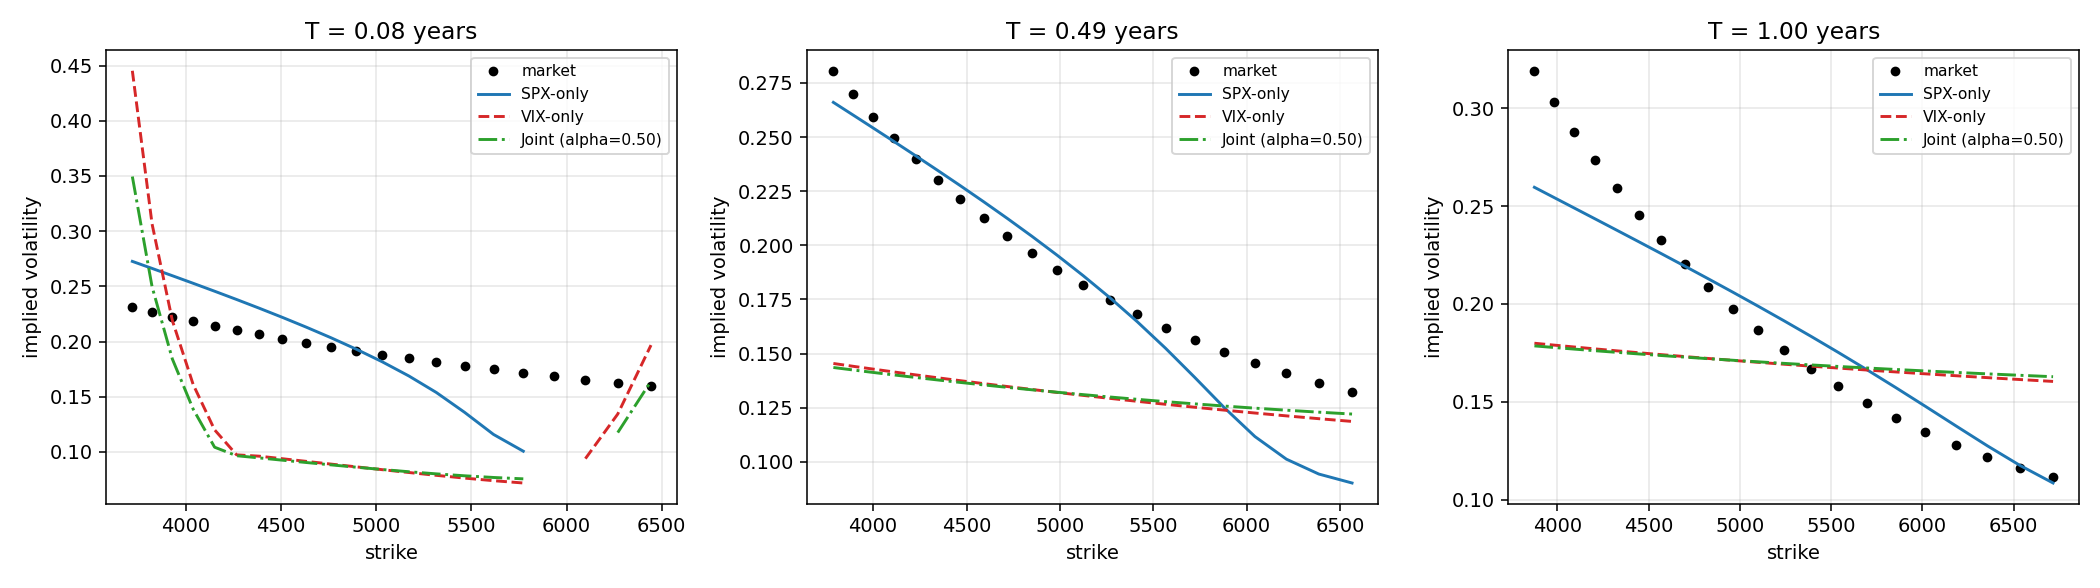
\includegraphics[width=0.88\textwidth]{figures/spx_smile_comparison.png}
    \caption{Comparison of SPX market and model-implied volatility smiles under different Heston calibration settings. The figure illustrates how SPX-only, VIX-only, and joint calibrations affect the fit to the SPX implied-volatility surface.}
    \label{fig:spx_smile_comparison}
\end{figure}

\begin{figure}[htbp]
    \centering
    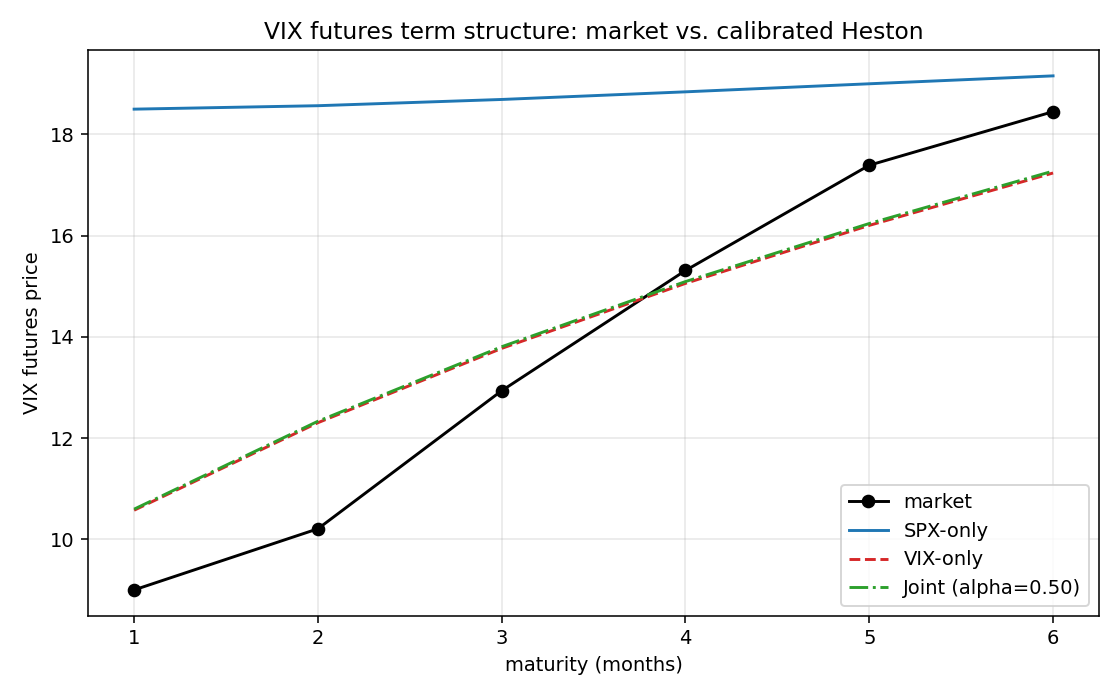
\includegraphics[width=0.88\textwidth]{figures/vix_futures_comparison.png}
    \caption{Comparison of market and model-implied VIX futures term structures under different calibration settings. The figure shows the difficulty of fitting VIX futures and SPX smiles simultaneously with a one-factor Heston model.}
    \label{fig:vix_futures_comparison}
\end{figure}

\begin{figure}[htbp]
    \centering
    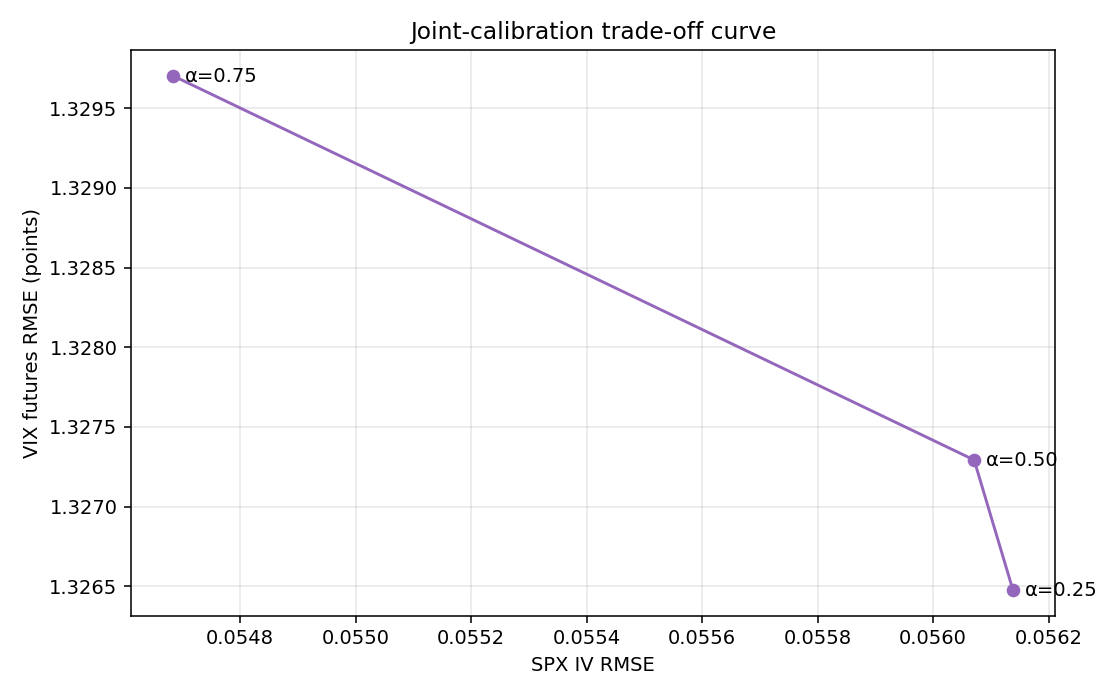
\includegraphics[width=0.82\textwidth]{figures/tradeoff_curve.png}
    \caption{Calibration trade-off between SPX implied-volatility RMSE and VIX futures RMSE. The figure visualises the structural limitation of the one-factor Heston model in joint SPX--VIX calibration.}
    \label{fig:tradeoff_curve}
\end{figure}

\subsection{Interpretation of Calibration Results}

The SPX-only calibration produces a strong fit to the SPX implied-volatility surface, with an SPX IV RMSE of \(0.0159\). However, the same parameter set produces a VIX futures RMSE of \(5.90\), indicating a poor fit to the VIX futures curve.

The VIX-only calibration produces a much better VIX futures RMSE of \(1.32\), but the SPX IV RMSE deteriorates to \(0.0711\). This means that the parameter set that fits the VIX futures curve does not reproduce the SPX volatility smile well.

The joint calibration with \(\alpha=0.50\) produces an SPX IV RMSE of \(0.0561\) and a VIX futures RMSE of \(1.33\). This result remains much closer to the VIX-only solution than to the SPX-only solution. The optimiser sacrifices SPX fit in order to keep the VIX futures curve close to the market.

Figures~\ref{fig:spx_smile_comparison}, \ref{fig:vix_futures_comparison}, and \ref{fig:tradeoff_curve} illustrate this trade-off visually. Together, they show that the one-factor Heston model can match one market dimension at a time, but struggles to fit the SPX smile and the VIX futures term structure simultaneously.

\subsection{Structural Implication}

The W6 calibration results support the central structural limitation discussed in the theory section: a one-factor Heston model can reproduce either the SPX smile or the VIX futures curve reasonably well, but not both simultaneously.

The SPX surface requires a strongly negative \(\rho\) and sufficient volatility-of-volatility to generate skew. The VIX futures curve is more directly controlled by the mean-reversion parameters and long-run variance level. Because a single variance factor must satisfy both markets at the same time, the model faces a structural trade-off.

This motivates the use of richer models in future work. Possible extensions include two-factor CIR models, forward-variance models, and rough-volatility models. These models introduce additional flexibility by decoupling short-term and long-term variance behaviour or by changing the regularity of the variance process.
\section{Results and Discussion}
\label{sec:results_discussion}

This section discusses the main results obtained across the completed W3--W8 components. The project begins with model-based numerical validation and then moves toward empirical volatility analysis, calibration, volatility-surface interpretation, and volatility risk premium backtesting.

The results should be interpreted in stages. W3 and W4 validate the numerical pricing framework under controlled model parameters. W5 connects the framework to market data and realised variance. W6 evaluates whether a one-factor Heston model can jointly fit SPX and VIX-related instruments. W7 studies the structural difference between VIX and SPX volatility surfaces. W8 evaluates the practical behaviour of a volatility risk premium strategy across regimes.

\subsection{W3--W4 Numerical Validation}

The first numerical validation compares the Monte Carlo engine from W3 with the COS pricing engine from W4. Both methods price the same model-implied VIX call under the same Heston/CIR parameter set. The benchmark parameters are
\begin{equation}
v_0=0.04,\qquad
\kappa=2,\qquad
\theta=0.04,\qquad
\sigma_v=0.5,
\end{equation}
with option maturity
\begin{equation}
T=\frac{30}{365},
\end{equation}
risk-free rate
\begin{equation}
r=0.03,
\end{equation}
and VIX option strike
\begin{equation}
K=20.
\end{equation}

The Monte Carlo engine simulates Heston stock and variance paths, computes realised variance, validates the realised variance against the analytical variance swap strike, and prices the model-implied VIX call. The COS engine uses the characteristic function of terminal CIR variance and computes the same expected payoff through a Fourier-cosine expansion.

The comparison is summarised in Table~\ref{tab:cos_mc_comparison}.

\begin{table}[htbp]
\centering
\begin{tabular}{lcc}
\toprule
Quantity & Value & Interpretation \\
\midrule
COS price & 2.008969 & Characteristic-function-based estimate \\
Monte Carlo price & 1.984952 & Simulation-based estimate \\
Absolute difference & 0.024017 & Difference between pricing engines \\
Relative difference & 1.21\% & Difference relative to Monte Carlo price \\
\bottomrule
\end{tabular}
\caption{Comparison between COS and Monte Carlo prices for the model-implied VIX call.}
\label{tab:cos_mc_comparison}
\end{table}

The absolute difference is
\begin{equation}
\mathrm{AbsError}
=
|C_0^{COS}-C_0^{MC}|
=
0.024017,
\end{equation}
and the relative difference is approximately
\begin{equation}
\mathrm{RelError}
=
\frac{|C_0^{COS}-C_0^{MC}|}{C_0^{MC}}
\approx
1.21\%.
\end{equation}

This result supports the numerical consistency of the two independently implemented pricing engines. Exact equality is not expected because Monte Carlo contains sampling and time-discretisation error, while the COS method contains truncation, finite-series approximation, and payoff-integration error.

\subsection{W5 Market Data and Volatility Risk Premium Findings}

The W5 stage extends the project from synthetic model testing to market-data analysis. The data pipeline collects VIX index levels, SPX index data, VIX futures settlement data, and a risk-free rate proxy. From SPX returns, realised variance is computed, while implied variance is approximated from the VIX index.

The volatility risk premium is estimated as
\begin{equation}
VRP_t
=
\frac{1}{12}
\left(
\frac{VIX_t}{100}
\right)^2
-
RV_{t,t+1M}.
\end{equation}
A positive value indicates that implied variance exceeds subsequently realised variance.

The W5 results support several stylised facts. VIX rises sharply during stress episodes, realised variance increases after market shocks, and the volatility risk premium is generally positive during calm periods. However, crisis periods may compress or reverse the premium. This behaviour is consistent with the interpretation of volatility as an insurance-like asset class: investors pay for protection in normal periods, while volatility sellers are compensated for bearing crash risk.

The W5 analysis also identifies the 2020 COVID shock and the 2022 inflation shock as important stress periods. In such regimes, implied volatility rises sharply, realised variance catches up after market moves, and the relationship between VIX changes and SPX returns becomes strongly negative.

\subsection{W6 Calibration Trade-Off}

The W6 calibration results show that the one-factor Heston model faces a structural difficulty when fitting both SPX and VIX markets. The SPX-only calibration fits the SPX implied-volatility surface well, with an SPX IV RMSE of \(0.0159\), but produces a VIX futures RMSE of \(5.90\). In contrast, the VIX-only calibration improves the VIX futures RMSE to \(1.32\), but the SPX IV RMSE deteriorates to \(0.0711\).

The joint calibration with \(\alpha=0.50\) produces an SPX IV RMSE of \(0.0561\) and a VIX futures RMSE of \(1.33\). This solution is closer to the VIX-only calibration than to the SPX-only calibration, suggesting that the joint objective sacrifices SPX smile fit to preserve the VIX futures fit.

This trade-off is economically meaningful. The SPX volatility smile is strongly influenced by negative stock-variance correlation and volatility-of-volatility. The VIX futures curve is more sensitive to the variance level, long-run variance, and mean-reversion speed. A single variance factor cannot easily satisfy both requirements at once.

\subsection{W7 Volatility Surface Analysis}

The W7 component analyses the structural difference between VIX and SPX implied-volatility surfaces. VIX options are options written on the VIX index itself. Their implied volatility is often interpreted as volatility-of-volatility because it reflects market expectations about the magnitude of future VIX movements.

Under the CIR variance process, terminal variance \(v_T\) follows a scaled non-central chi-square distribution. Since this distribution is positive and right-skewed, the model-implied VIX inherits a right-skewed distribution. This provides a mathematical explanation for the positive skew observed in VIX option prices.

The W7 results show that VIX and SPX smiles have opposite skew directions. The VIX smile has positive skew, meaning that out-of-the-money VIX calls are relatively expensive. The SPX smile has negative skew, meaning that out-of-the-money SPX puts are relatively expensive. This contrast is summarised in Table~\ref{tab:w7_smile_comparison}.

\begin{table}[htbp]
\centering
\begin{tabular}{lll}
\toprule
Feature & VIX Options & SPX Options \\
\midrule
Skew direction & Positive/right skew & Negative/left skew \\
Expensive wing & OTM calls & OTM puts \\
Underlying tail & Fat right tail & Fat left tail \\
Main crisis exposure & Volatility spikes & Equity drawdowns \\
Model source & Non-central \(\chi^2\) variance distribution & Negative Heston correlation \(\rho\) \\
Investor behaviour & VIX calls as tail hedge & SPX puts as downside protection \\
\bottomrule
\end{tabular}
\caption{Structural comparison between VIX and SPX implied-volatility smiles.}
\label{tab:w7_smile_comparison}
\end{table}

The reported one-month VIX 25-delta risk reversal is approximately \(+11.49\) volatility points, while the corresponding SPX 25-delta risk reversal is approximately \(-9.55\) volatility points. The opposite signs confirm the different economic roles of the two option markets. VIX calls insure against volatility spikes, while SPX puts insure against market declines.

This result also connects W7 to the earlier Heston model discussion. Negative stock-variance correlation explains the SPX downside skew, while the positive and right-skewed distribution of terminal variance explains the VIX upside skew.

\subsection{W8 Volatility Risk Premium Backtest}

The W8 component evaluates the practical behaviour of a volatility risk premium strategy. The generated outputs include backtest plots, daily and monthly P\&L summaries, regime-level metrics, beta decomposition, and risk dashboards.

Figure~\ref{fig:w8_backtest} shows the cumulative behaviour of the W8 volatility risk premium backtest.

\begin{figure}[htbp]
    \centering
    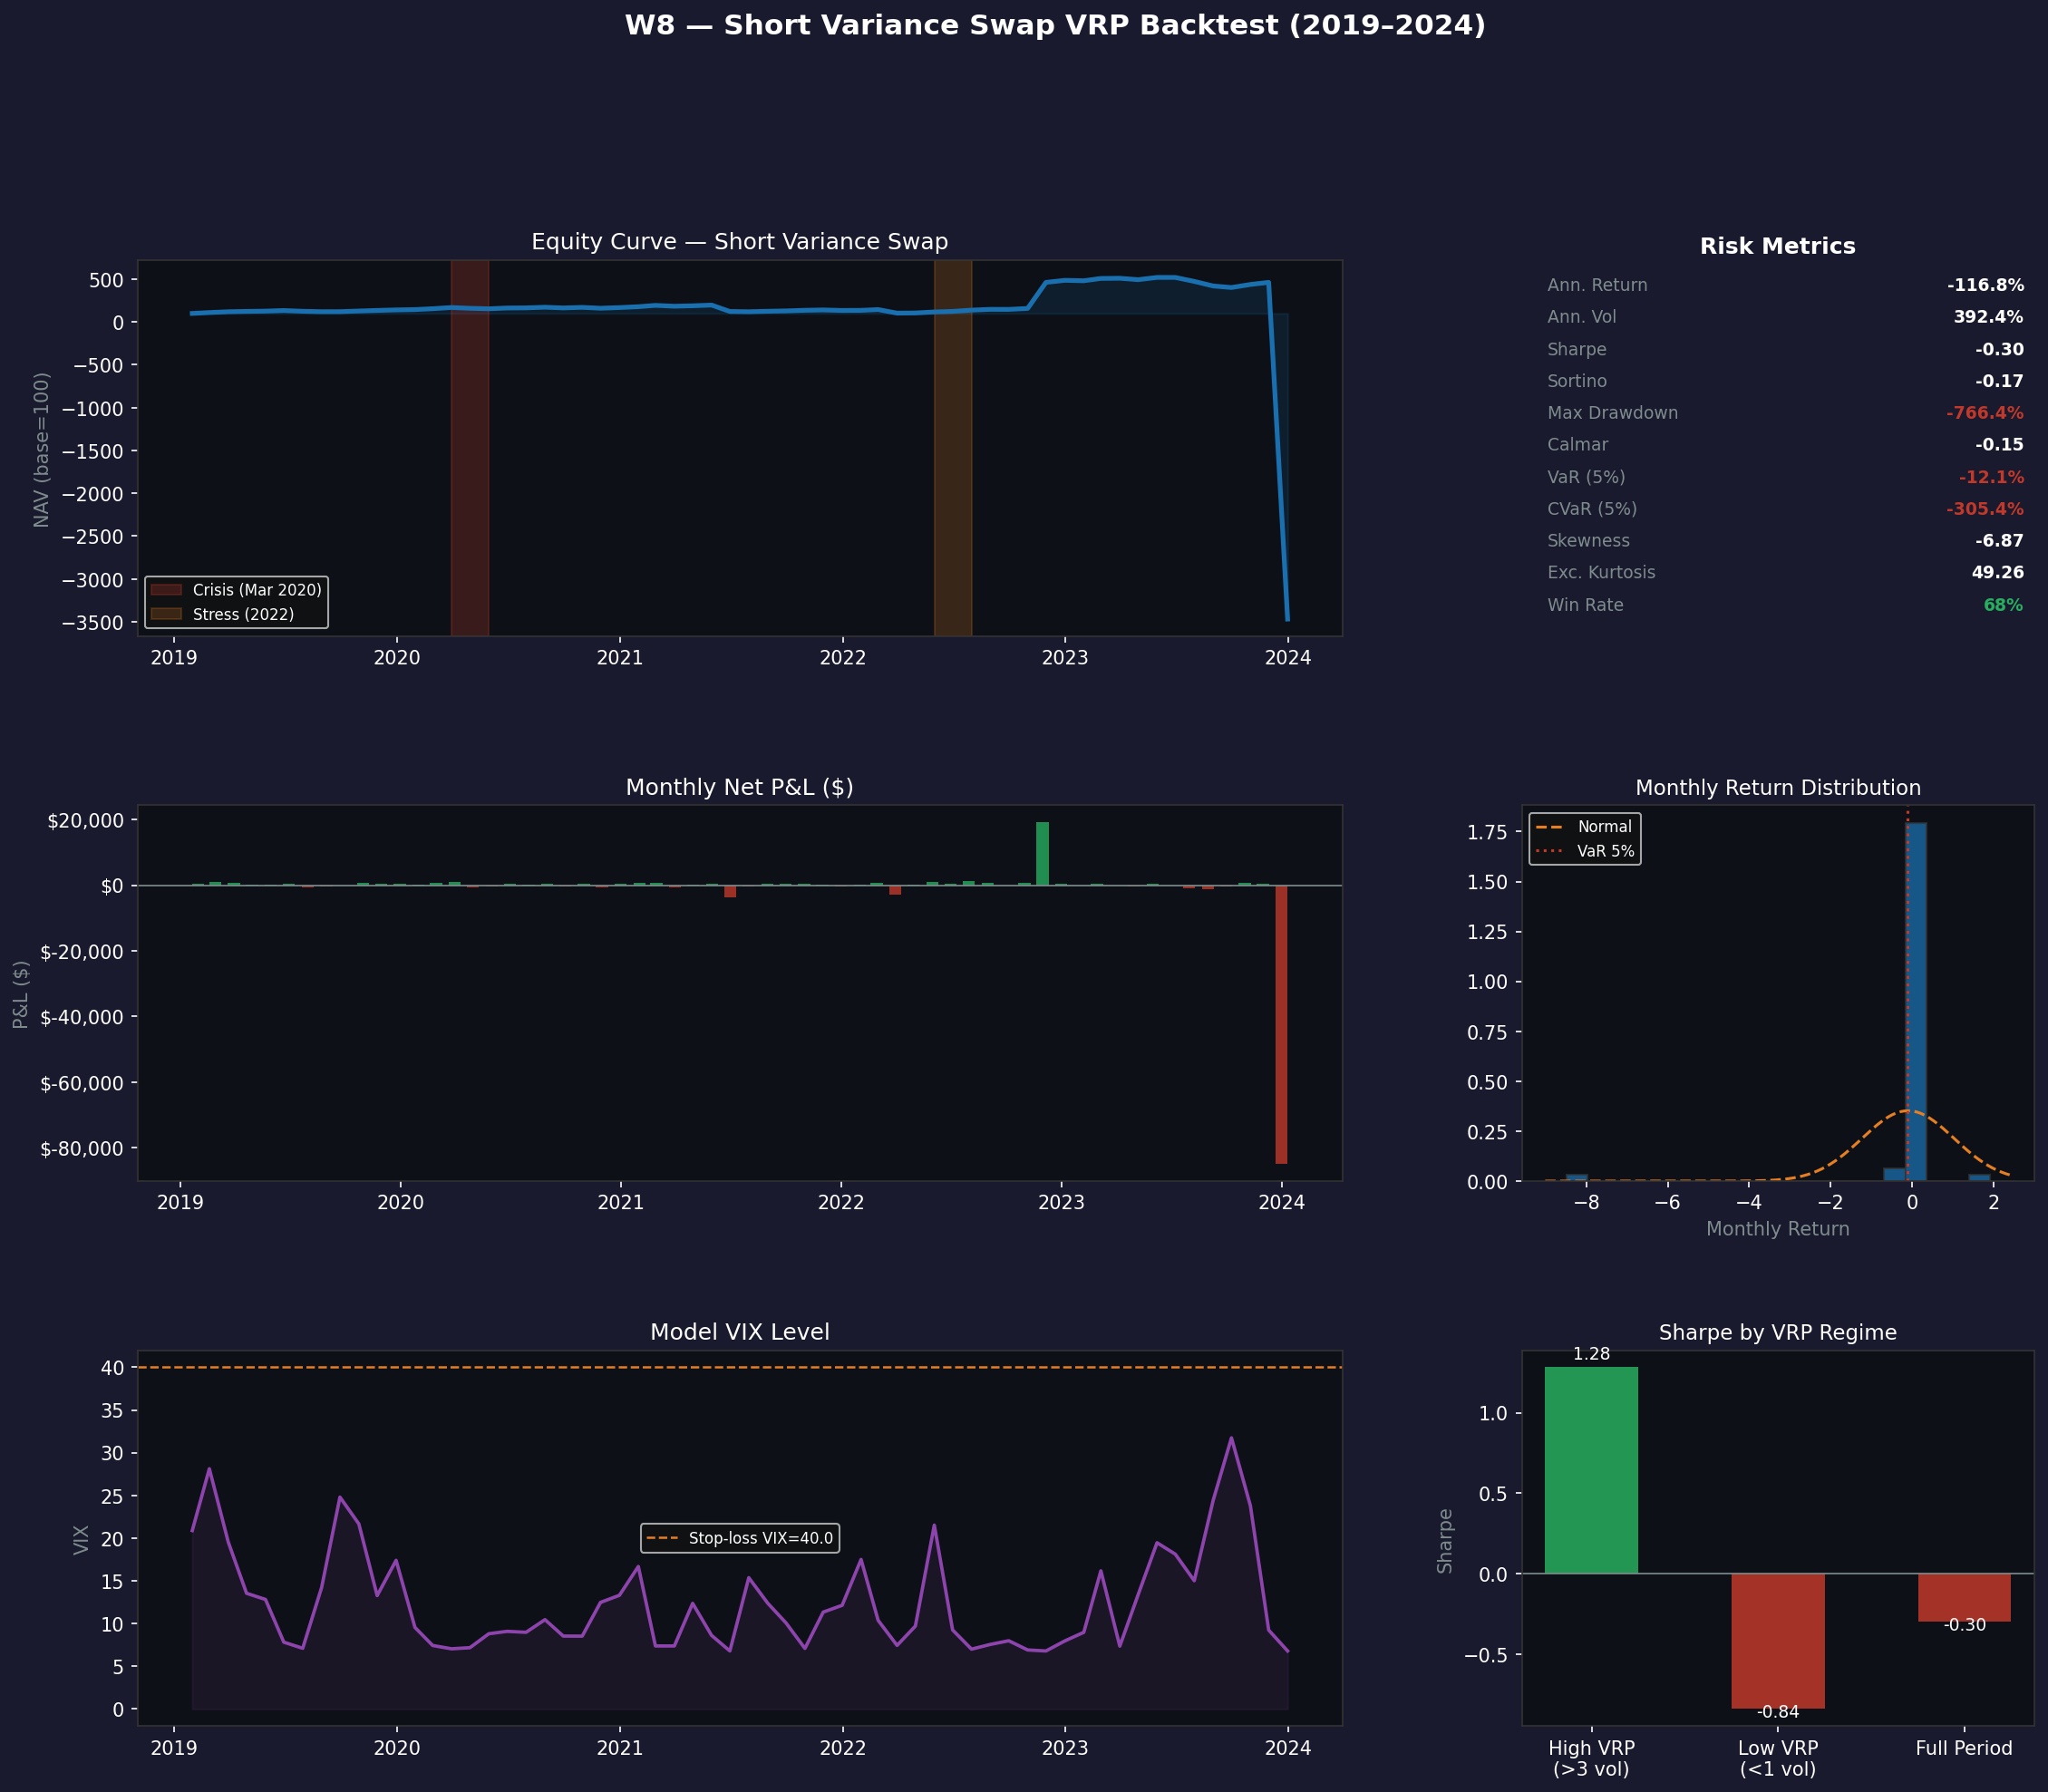
\includegraphics[width=0.88\textwidth]{figures/w8_backtest.png}
    \caption{Backtest performance of the volatility risk premium strategy. The figure summarises the cumulative behaviour of the strategy across the analysed period.}
    \label{fig:w8_backtest}
\end{figure}

Figure~\ref{fig:w8_daily_pnl} shows the daily P\&L behaviour of the strategy.

\begin{figure}[htbp]
    \centering
    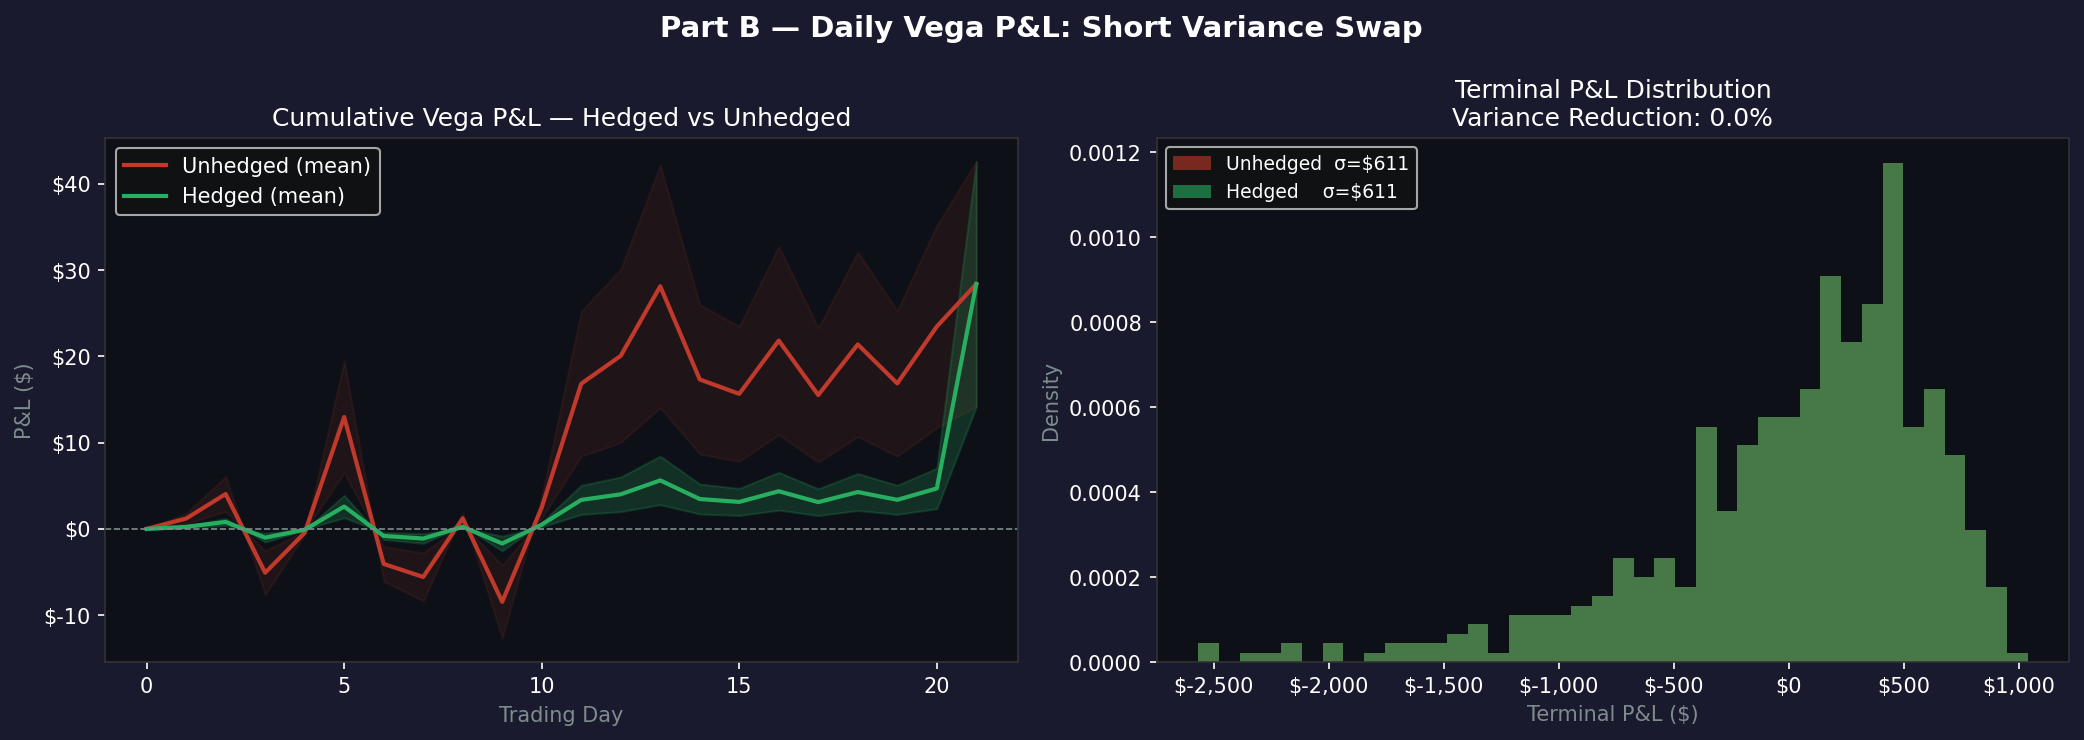
\includegraphics[width=0.88\textwidth]{figures/w8_daily_pnl.png}
    \caption{Daily P\&L of the volatility risk premium strategy. The figure illustrates the time-series behaviour and stress sensitivity of the strategy.}
    \label{fig:w8_daily_pnl}
\end{figure}

The W8 metrics are summarised in Table~\ref{tab:w8_vrp_metrics}.

\begin{table}[htbp]
\centering
\begin{tabular}{lccc}
\toprule
Metric & Full Period & High VRP Regime & Low VRP Regime \\
\midrule
Annual return & -- & 2.154 & -- \\
Annual volatility & 3.925 & 1.218 & 6.102 \\
Sharpe ratio & -- & 1.768 & -- \\
Maximum drawdown & -7.664 & 0.000 & -2.763 \\
VaR 5\% & -0.121 & 0.039 & -0.369 \\
CVaR 5\% & -3.054 & 0.035 & -4.438 \\
Skewness & -7.044 & 5.264 & -4.775 \\
Kurtosis & 53.708 & 27.794 & 22.855 \\
Observations & 60 & 28 & 23 \\
\bottomrule
\end{tabular}
\caption{W8 volatility risk premium backtest metrics across regimes. Empty entries correspond to metrics not reported in the generated output file.}
\label{tab:w8_vrp_metrics}
\end{table}

The high-VRP regime shows the strongest risk-adjusted profile, with a reported Sharpe ratio of approximately \(1.77\), annual return of approximately \(2.15\), and annual volatility of approximately \(1.22\). However, the full-period metrics also show strong negative skewness and high kurtosis, indicating that volatility-selling strategies carry significant tail risk.

Figure~\ref{fig:w8_metrics_dashboard} summarises the W8 strategy metrics visually.

\begin{figure}[htbp]
    \centering
    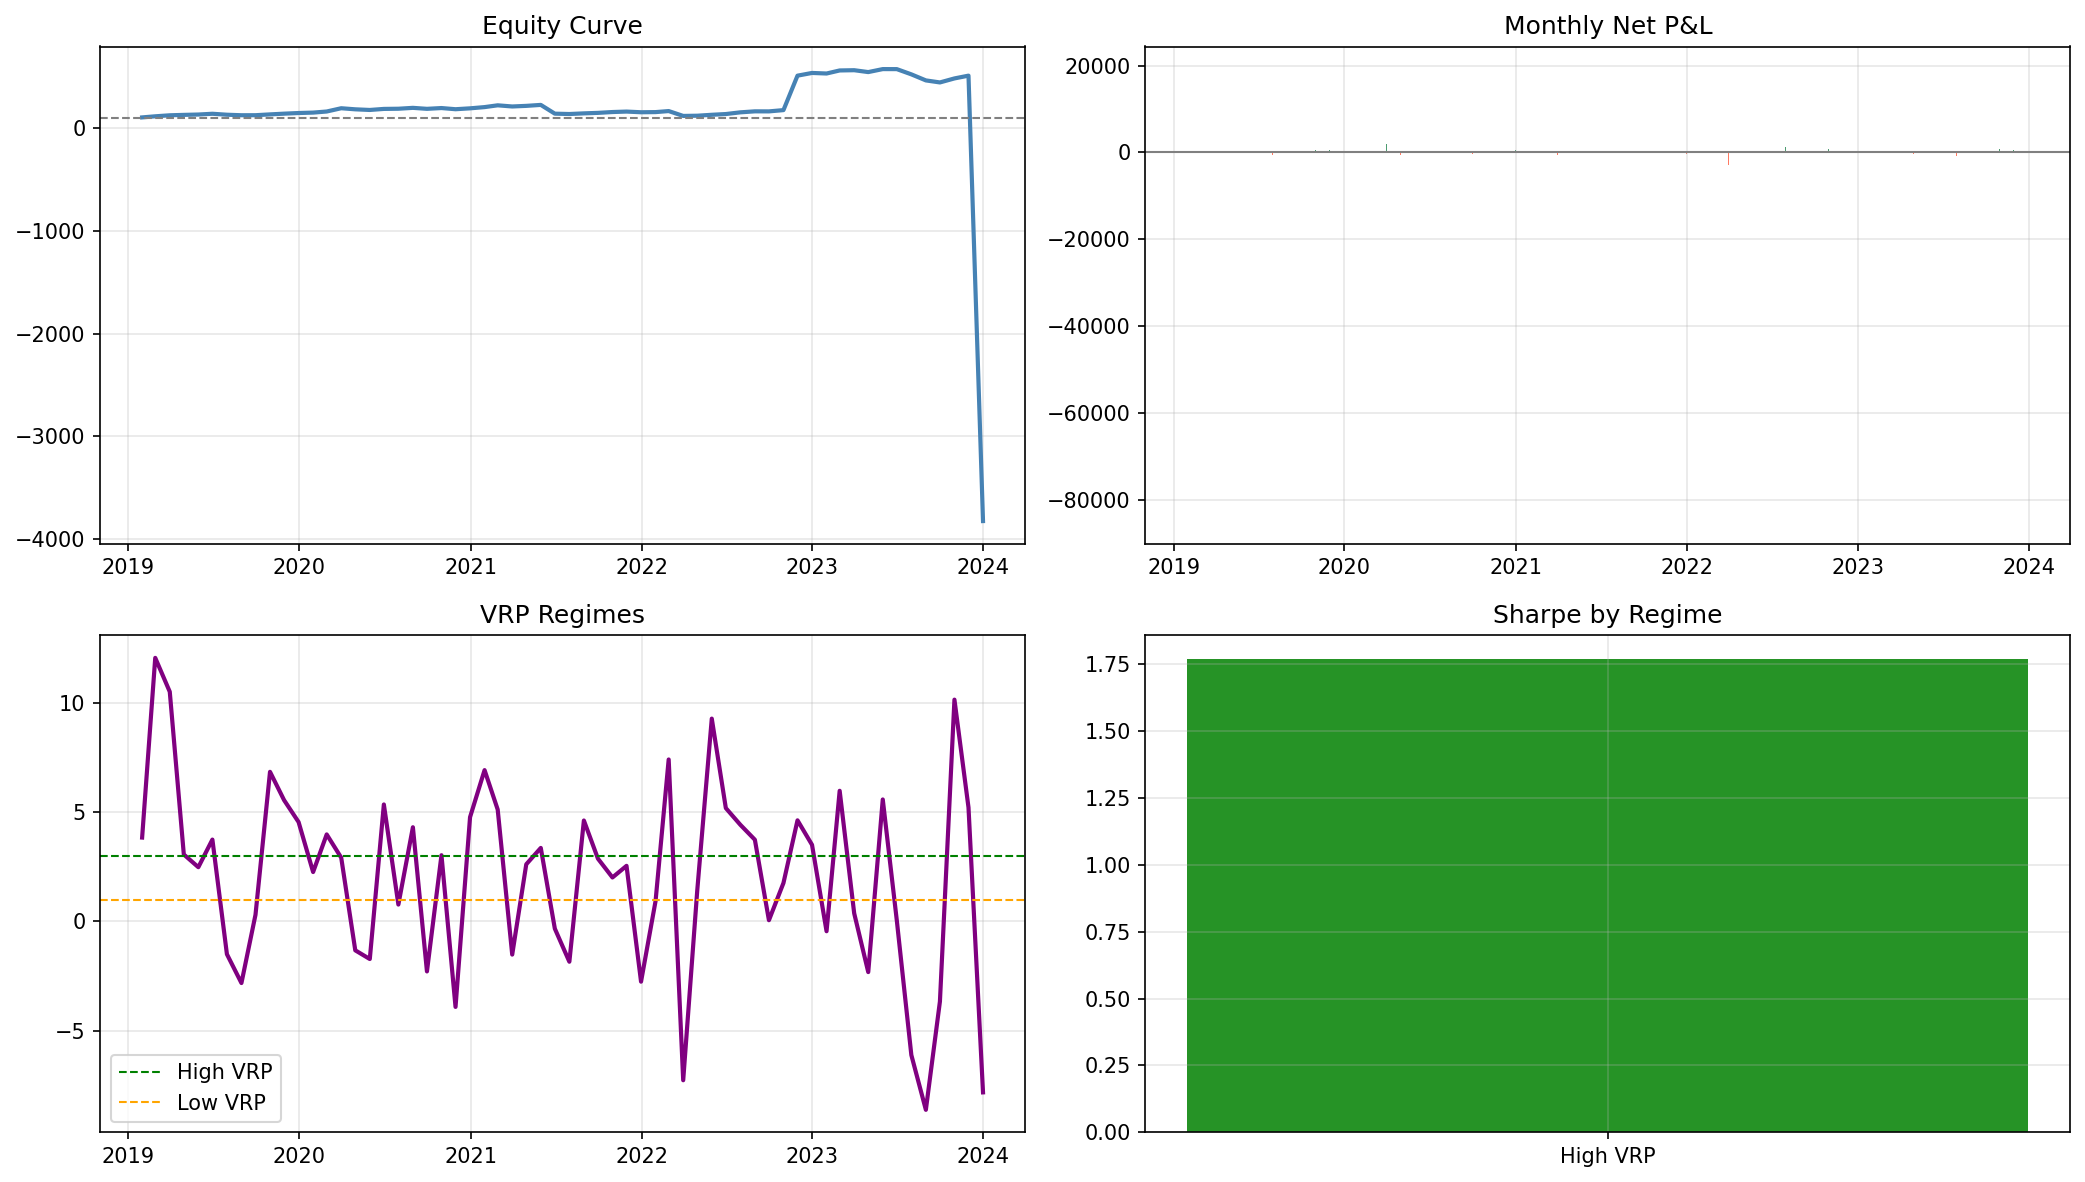
\includegraphics[width=0.88\textwidth]{figures/w8_metrics_dashboard.png}
    \caption{W8 risk and performance dashboard for the volatility risk premium strategy. The dashboard summarises return, volatility, drawdown, and tail-risk behaviour across regimes.}
    \label{fig:w8_metrics_dashboard}
\end{figure}

The W8 results are consistent with the economic interpretation developed earlier in the paper. Volatility risk premium strategies can perform well when implied variance is high relative to expected realised variance, but they remain exposed to severe losses during volatility spikes and crisis periods. Therefore, performance evaluation must include not only average returns and Sharpe ratios, but also drawdowns, tail losses, skewness, and regime dependence.

\subsection{Model-Free Hedging Output}

The W8 outputs also include a model-free hedge diagnostic. Figure~\ref{fig:w8_model_free_hedge} summarises the generated hedge output.

\begin{figure}[htbp]
    \centering
    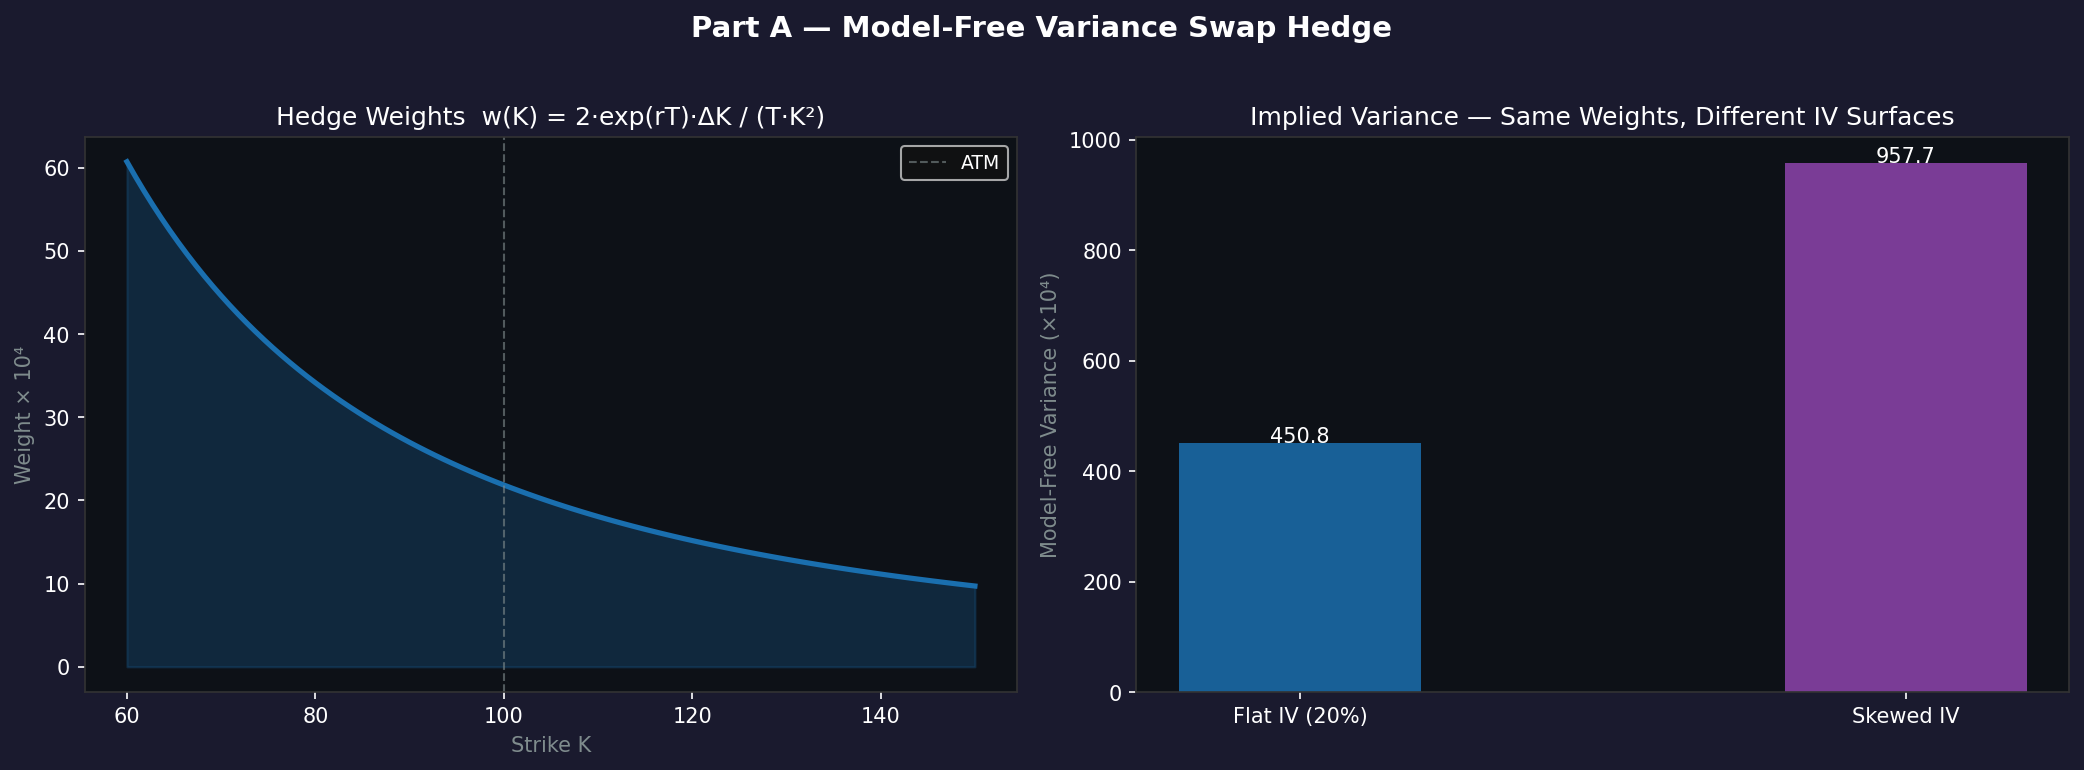
\includegraphics[width=0.88\textwidth]{figures/w8_model_free_hedge.png}
    \caption{Model-free hedging diagnostic generated in W8. The figure provides an additional view of strategy risk management and hedge behaviour.}
    \label{fig:w8_model_free_hedge}
\end{figure}

The inclusion of hedge diagnostics is important because volatility strategies cannot be evaluated only by their average return. A strategy may appear profitable in normal regimes but fail during volatility spikes if hedging is weak or if tail exposure is not controlled.

\subsection{Integrated Interpretation across W3--W8}

The completed project forms a coherent pipeline. W3 provides a Monte Carlo simulation engine for stochastic variance and VIX-type payoffs. W4 provides a faster COS pricing engine based on the CIR characteristic function. W5 introduces real market data and volatility risk premium estimation. W6 demonstrates the calibration trade-off between SPX and VIX markets. W7 explains the structural difference between SPX and VIX volatility smiles. W8 evaluates the practical risk-return behaviour of a volatility risk premium strategy.

The central conclusion is that volatility can be treated as a tradable asset class, but it requires careful modelling. Simple one-factor stochastic volatility models are useful for theory and implementation, but they face limitations in joint calibration and empirical strategy design. Numerical pricing, calibration, smile analysis, and backtesting must therefore be interpreted together rather than as separate tasks.
\section{Conclusion}
\label{sec:conclusion}

This project studied volatility as a tradable asset class through variance swaps, model-implied VIX derivatives, volatility-surface analysis, calibration, and volatility risk premium backtesting. The main objective was to connect the theoretical structure of volatility-linked products with working numerical methods and empirical analysis.

The first part of the project reviewed the role of volatility derivatives in modern financial markets. Variance swaps, VIX futures, and VIX options provide direct exposure to volatility and variance rather than only to the direction of the underlying asset. This motivates a modelling framework in which variance is treated as a stochastic state variable. The Heston model was used as the baseline framework because its variance process is mean-reverting, non-negative in continuous time, and analytically tractable enough for both simulation and characteristic-function-based pricing.

The theoretical part derived the key formulas required for the numerical implementation. The fair variance swap strike was obtained from the expected integrated variance under the Heston/CIR variance process. The project also constructed a model-implied VIX proxy based on the conditional expectation of future variance. This distinction is important because the proxy used in the project is not the official Cboe VIX index. Instead, it is a Heston-implied quantity of the form
\[
\widetilde{\mathrm{VIX}}_T
=
100\sqrt{A_\Delta+B_\Delta v_T}.
\]
This representation allowed VIX-type payoffs to be expressed as functions of terminal variance.

The W3 component implemented the Monte Carlo engine. It simulated Heston stock and variance paths using a full-truncation Euler scheme, computed realised variance from squared log returns, and compared the simulated realised variance with the analytical Heston variance swap strike. This comparison served as the first validation step for the simulation engine. The same Monte Carlo framework was also used to price a model-implied VIX call by transforming terminal variance into VIX and averaging discounted payoffs.

The W4 component implemented the CIR-based COS pricing engine. The method used the characteristic function of terminal CIR variance and approximated the expected payoff through a Fourier-cosine expansion. This provided a deterministic semi-analytical benchmark for the Monte Carlo VIX call price. The COS framework was also used for density recovery, VIX call and put pricing, VIX futures term-structure calculation, and convergence checks with respect to the number of terms and truncation interval.

The numerical comparison between the Monte Carlo and COS engines showed close agreement under the same parameter set. The reported COS price was approximately \(2.008969\), while the Monte Carlo price was approximately \(1.984952\). The absolute difference was \(0.024017\), corresponding to a relative difference of about \(1.21\%\). This result supports the internal consistency of the two independently implemented pricing methods.

The W5 component extended the project to market data. It introduced VIX index data, SPX market data, VIX futures data, realised variance estimation, implied variance approximation, volatility risk premium computation, and crisis-period analysis. The empirical findings confirmed several common volatility-market patterns: VIX rises during stress, implied variance is often higher than future realised variance in calm regimes, and volatility risk premium behaviour changes during crisis periods.

The W6 component implemented joint SPX--VIX calibration. The results showed a structural limitation of the one-factor Heston model. SPX-only calibration fitted the SPX implied-volatility surface better, while VIX-only calibration fitted the VIX futures curve better. The joint calibration did not dominate both single-market calibrations. This confirms that one variance factor is often insufficient to fit both SPX and VIX markets simultaneously.

The W7 component analysed volatility surfaces. The comparison between VIX and SPX smiles showed that VIX options tend to exhibit positive skew, while SPX options tend to exhibit negative skew. This difference has both mathematical and economic explanations. Under the CIR model, terminal variance is positive and right-skewed, which supports the right-skewed VIX distribution. In SPX options, negative stock-variance correlation and demand for downside protection support the left-skewed volatility smile.

The W8 component evaluated volatility risk premium backtesting and risk metrics. The results showed that high-VRP regimes can produce attractive risk-adjusted performance, but the full-period results also reveal substantial tail risk through drawdowns, negative skewness, and high kurtosis. This confirms that volatility-selling strategies cannot be evaluated only by average return or Sharpe ratio. Tail risk, crisis exposure, and regime dependence are central to the economic interpretation.

The main contribution of the project is therefore a complete research pipeline from theory to implementation and empirical testing. The project includes literature review, mathematical derivations, Monte Carlo simulation, COS pricing, data collection, calibration, volatility-surface analysis, and VRP backtesting. The work also includes a modular codebase, notebooks, diagnostic outputs, and a test suite that validates the main numerical components.

Several limitations remain. First, the official Cboe VIX methodology is more complex than the model-implied VIX proxy used in the theoretical and pricing sections. Second, the one-factor Heston/CIR model cannot fully capture the joint behaviour of SPX and VIX markets. Third, some empirical components rely on available data pipelines, cached snapshots, or synthetic fallback surfaces when live data are unavailable. Fourth, the COS method depends on truncation intervals and numerical payoff integration. Finally, volatility risk premium backtests remain sensitive to regime definitions, transaction costs, and crisis-period assumptions.

Future work should focus on improving both the model and the empirical strategy design. On the modelling side, possible extensions include two-factor CIR models, forward-variance models, rough Heston dynamics, and jump-diffusion specifications. These models may provide more flexibility for fitting SPX smiles, VIX futures, and VIX option surfaces simultaneously. On the numerical side, closed-form COS payoff coefficients and adaptive truncation rules could improve efficiency and accuracy. On the empirical side, future work should incorporate live market data, transaction costs, robust hedging rules, and more detailed stress testing.

Overall, the completed project demonstrates that volatility can be studied as a tradable asset class through a combination of stochastic modelling, numerical pricing, calibration, surface analysis, and backtesting. The Monte Carlo and COS engines provide the numerical foundation, the calibration results reveal the limitations of a one-factor model, the volatility-surface analysis explains the difference between VIX and SPX options, and the VRP backtest connects the modelling framework to investment and risk-management implications.

\bibliographystyle{apalike}
\bibliography{references}

\end{document}